
\documentclass{article}
\usepackage{amsmath,amssymb,amsfonts}
\usepackage{graphicx}
\usepackage{geometry}
\usepackage{authblk}
\usepackage[utf8]{inputenc}
\usepackage{hyperref}
\usepackage{caption}
\usepackage{subcaption}
\usepackage{booktabs}
\usepackage{array}
\usepackage{enumitem}
\usepackage{tikz}
\usetikzlibrary{trees}
\usepackage{rotating} % Used for rotating the large matrix in the appendix if necessary

% Setup geometry
\geometry{a4paper, margin=1in}

% Title and Author Information
\title{A Probabilistic Solution to High-Dimensional Continuous-Time Macro and Finance Models}
\author{Ji Huang\thanks{I am incredibly grateful to Han Jiequn for answering numerous questions on their algorithms and BSDES. My CUHK colleague Vinci Chow provided tremendous technical support on Tensorflow. Yu Jinghai and Geng Bojun offered superb research assistance. For insightful feedbacks, I would like to thank Hengjie Ai, Ken Judd, Wenlan Luo, Jianjun Miao, Galo Nūno, Shi Qiu, Yuliy Sannikov as well as seminar and conference participants of Zhejiang University, Shanghai JiaoTong, Fudan, SHUFE, Fudan Workshop on Economic Dynamics 2023, CICM 2023, AMES 2023, NASM 2023, SITE 2023 New Frontier in Asset Pricing, CESifo Macro Money, and International Finance 2023, CICF 2024, et al. My research benefits from the financial support of the General Research Fund of Hong Kong SAR (project number: 14501019). Contact Details: 9/F Esther Lee Building, The Chinese University of Hong Kong, Shatin, Hong Kong, China. Email:jihuang@cuhk.edu.hk.}}
\affil{The Chinese University of Hong Kong}
\date{August 5, 2025}

\begin{document}

\maketitle

\begin{abstract}
This paper introduces the probabilistic formulation of continuous-time economic models: forward stochastic differential equations (SDEs) govern the dynamics of backward-looking variables, while backward SDEs capture those of forward-looking variables. Deep learning streamlines the search for probabilistic solutions, which are less sensitive to the "curse of dimensionality." The paper proposes two types of algorithms and assesses their accuracy and computational speed by applying them to a multi-country model with an explicit solution under symmetric states. Numerical experiments indicate that as the model's dimensionality increases, the computational speed of the partial differential equation approach deteriorates exponentially, whereas that of the probabilistic approach declines only linearly.
\end{abstract}

\noindent \textbf{JEL Classification:} C63, G21, E44

\noindent \textbf{Keywords:} backward stochastic differential equation, deep learning, the curse of dimensionality, economic dynamics

\clearpage

\section*{Introduction}

With the recent success of artificial intelligence, economists have begun applying deep learning to solve high-dimensional models including those in the continuous-time setting e.g., Duarte, Duarte and Silva (2024), Fernández-Villaverde, Hurtado and Nuno (2022), and papers in the literature session. Thus far, all of these papers employ the analytic formulation and solve for equilibrium using partial differential equations (PDEs). Although deep learning provides a powerful toolbox for approximating high-dimensional functions, solving PDEs still suffers from the curse of dimensionality, particularly due to the Hessian matrices critical components in PDEs that describe models driven by diffusion processes.

In this paper, I introduce Backward Stochastic Differential Equations (BSDEs) the probabilistic counterpart to PDEs to a general audience in economics, and more importantly, I highlight their computational advantages, especially the fact that they bypass the need to compute Hessian matrices. The development of BSDEs began with the seminal paper by Pardoux and Peng (1990). My work is largely inspired by Han, Jentzen and E (2018), the first paper to apply deep learning to high-dimensional BSDEs and the corresponding PDES.

Due to its technical difficulty, I will first present the key intuition and terminology of BSDES using a two-period binomial tree model, in which the European call option's payoff at expiration is given by $Y_{j}=\max\{0,X_{j}-K\}$, j = uu, ud, du, dd. The no-arbitrage condition implies that the option price equals the value of the replicating portfolio $(B_{u},S_{u})$, where $B_{u}$ is the risk-free saving and $S_{u}$ is the number of shares of the underlying stock. Replicating the payoff from node u onward requires that $(B_{u},S_{u})$ solves the following 2-by-2 linear system:
\begin{equation}
Y_{uu}=RB_{u}+X_{uu}S_{u}: \quad Y_{ud}=RB_{u}+X_{ud}S_{u}
\label{eq:1}
\end{equation}
The no-arbitrage condition then yields the option price at node u as $Y_{u}=B_{u}+X_{u}S_{u}$. The same procedure applies to obtain $Y_{d}$ and $Y_{0}$. Next, I reinterpret the procedure for solving $\{Y_{i},i=0,u,d\}$ through the lens of a BSDE.

\begin{figure}[h]
    \centering
    \begin{subfigure}[b]{0.45\textwidth}
        \centering
        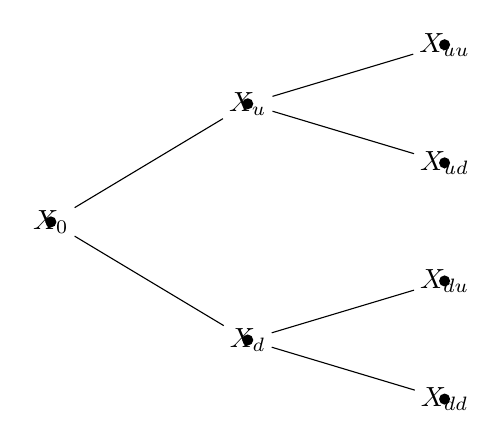
\begin{tikzpicture}[
            grow=right,
            level distance=2.5cm,
            level 1/.style={sibling distance=3cm},
            level 2/.style={sibling distance=1.5cm},
            % edge from parent/.style={draw, -latex},
            every node/.style={inner sep=2pt}
        ]
        \node (X0) {$X_0$}
            child {node (Xd) {$X_d$}
                child {node (Xdd) {$X_{dd}$}}
                child {node (Xdu) {$X_{du}$}}
            }
            child {node (Xu) {$X_u$}
                child {node (Xud) {$X_{ud}$}}
                child {node (Xuu) {$X_{uu}$}}
            };
        % Add dots at nodes
        \foreach \nodename in {X0, Xu, Xd, Xuu, Xud, Xdu, Xdd}
            \fill (\nodename) circle (2pt);
        \end{tikzpicture}
        \caption{Stock price tree}
    \end{subfigure}
    \hfill
    \begin{subfigure}[b]{0.45\textwidth}
        \centering
        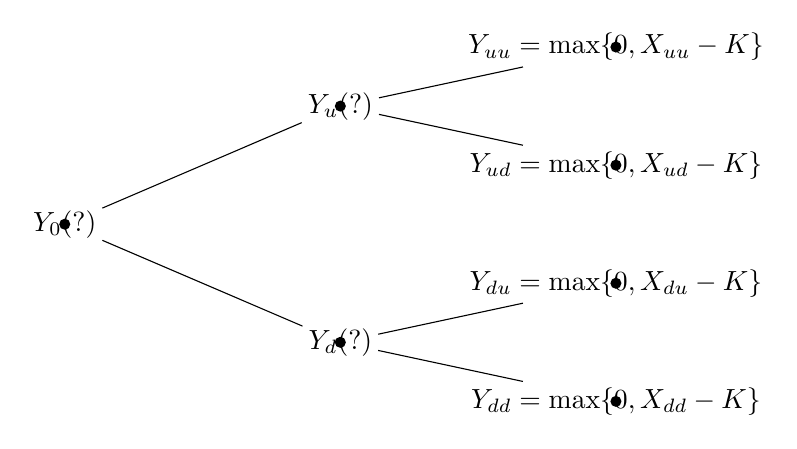
\begin{tikzpicture}[
            grow=right,
            level distance=3.5cm,
            level 1/.style={sibling distance=3cm},
            level 2/.style={sibling distance=1.5cm},
            % edge from parent/.style={draw, -latex},
            every node/.style={inner sep=2pt}
        ]
        \node (Y0) {$Y_0(?)$}
            child {node (Yd) {$Y_d(?)$}
                child {node (Ydd) {$Y_{dd} = \max\{0, X_{dd}-K\}$}}
                child {node (Ydu) {$Y_{du} = \max\{0, X_{du}-K\}$}}
            }
            child {node (Yu) {$Y_u(?)$}
                child {node (Yud) {$Y_{ud} = \max\{0, X_{ud}-K\}$}}
                child {node (Yuu) {$Y_{uu} = \max\{0, X_{uu}-K\}$}}
            };
        % Add dots at nodes
        \foreach \nodename in {Y0, Yu, Yd, Yuu, Yud, Ydu, Ydd}
            \fill (\nodename) circle (2pt);
        \end{tikzpicture}
        \caption{Option value tree}
    \end{subfigure}
    \caption{Binomial tree}
    \label{fig:1}
\end{figure}

Unlike Forward SDEs, the initial value $Y_{0}$ is determined as part of the solution implied by the terminal condition in a Backward SDE. More precisely, a BSDE's solution refers to the sequence of pairs $(Y_{i},S_{i})$, i = 0, u. d. Each pair solves a 2-by-2 linear system, and these three systems, together with the terminal condition, constitute a BSDE.

\clearpage

Consider node u: the pair $(Y_{u},S_{u})$ is the solution of the linear system
\begin{align*}
Y_{uu}&=RY_{u}+(X_{uu}-RX_{u})S_{u} \\
Y_{ud}&=RY_{u}+(X_{ud}-RX_{u})S_{u}
\end{align*}
which is derived by substituting $B_{u}$ in equations (\ref{eq:1}) with $Y_{u}-X_{u}S_{u}$. The pair $(Y_{u},S_{u})$ can be interpreted as the projection of the vector $(Y_{uu},Y_{ud})$ onto the plane spanned by (R, R) and $(X_{uu}-RX_{u},X_{ud}-RX_{u})$. The latter vector captures the risk of the underlying stock, and its coefficient $S_{u}$ serves as the control that ensures the portfolio's payoff matches the option's payoff. Similar 2-by-2 linear systems can be constructed at nodes d and 0, yielding the solution pairs $(Y_{d},S_{d})$ and $(Y_{0},S_{0})$, respectively.

Next, I introduce BSDEs using the continuous-time version of the same option pricing model. Suppose the short rate is a constant r and the underlying stock price $X_{t}$ follows the SDE given in (\ref{eq:2}). The no-arbitrage condition implies that the option price equals the value of its replicating portfolio $Y_{t}$ whose dynamic budget constraint is specified by the SDE in (\ref{eq:3}):
\begin{align}
dX_{t}&=X_{t}(\mu dt+\sigma dW_{t}), \quad X_{0}=x. \label{eq:2} \\
dY_{t}&=(rY_{t}+(\mu-r)X_{t}S_{t})dt+\sigma X_{t}S_{t}dW_{t}, \quad Y_{T}=\max\{0,X_{T}-K\}. \label{eq:3}
\end{align}
SDE (\ref{eq:3}) cannot be solved forward in time even if $Y_{0}$ is given because its evolution depends on the replicating strategy $\{S_{t}\}_{t\ge0}$. Thus, (\ref{eq:3}) is a Backward SDE with terminal condition $Y_{T}=\max\{0,X_{T}-K\}$. The process $\{Y_{t}\}_{t\ge0}$ must be solved backward along with $\{S_{t}\}_{t\ge0}$.

To connect with the binomial tree example, consider the time discretization of BSDE (\ref{eq:3}):
\begin{align*}
Y_{t+\Delta}&=(1+r\Delta)Y_{t}+((\mu\Delta+\sigma(W_{t+\Delta}-W_{t}))X_{t}-r\Delta X_{t})S_{t} \\
&=(1+r\Delta)Y_{t}+(X_{t+\Delta}-(1+r\Delta)X_{t})S_{t},
\end{align*}
where each realization of $W_{t+\Delta}$ determines $X_{t+\Delta}$ via SDE (\ref{eq:2}) and also determines $Y_{t+\Delta}$ either via the terminal condition on $Y_{T}$ if $t+\Delta=T$ or via backward induction along the path $\{X_{s}\}_{t+\Delta\le s<T}.$\footnote{Recall that $Y_{u}$ and $Y_{d}$ in the linear system at period 0 were solved using $Y_{uu}$ and $Y_{ud}$ which were obtained from the linear systems at nodes u and d in period 1.} At time t, the pair $(Y_{t},S_{t})$ is the solution of a system of linear equations, each corresponding to a realization of $W_{t+\Delta}$. In summary, the option pricing model is specified by the Forward-Backward SDE system (\ref{eq:2})-(\ref{eq:3}). Let $y(t,X_{t})$ and $s(t,X_{t})$ denote its solution pair.

There are two approaches to solving for $y(t,X_{t})$ and $s(t,X_{t})$: the analytic (PDE) approach and the probabilistic (BSDE or Monte Carlo) approach. Following the PDE approach, apply Itô's formula to $Y_{t}=y(t,X_{t})$:
\[
dY_{t}=\left(y_{t}(t,X_{t})+y_{x}(t,X_{t})\mu X_{t}+\frac{1}{2}y_{xx}(t,X_{t})\sigma^{2}X_{t}^{2}\right)dt+y_{x}(t,X_{t})\sigma X_{t}dW_{t}.
\]
Matching coefficients on $dW_{t}$ implies $s(t,x)=y_{x}(t,x)$, and matching coefficients on dt yields:
\begin{equation}
y_{t}(t,x)+rxy_{x}(t,x)+\frac{1}{2}\sigma^{2}x^{2}y_{xx}(t,x)=ry(t,x).
\label{eq:4}
\end{equation}

\clearpage

Combined with the terminal condition $y(T,x)=\max\{0,x-K\}$ this PDE characterizes the solution pair $y(t,X_{t})$ and $s(t,X_{t})$. Numerically solving for $y(t,X_{t})$ becomes challenging when the state variable $X_{t}$ is high-dimensional for two reasons: the difficulty of approximating a high-dimensional function and the computational cost of evaluating the Hessian matrix $y_{xx}(t,x)$. The enormous industrial success of deep learning suggests that neural network-based function spaces may address the first challenge. However, the second challenge remains a binding constraint that limits economists from exploring a wider range of models, to which the probabilistic approach can offer significant advantages.

The probabilistic (or Monte Carlo) approach has been widely used in derivative pricing. Next, I introduce how to combine deep learning with the probabilistic approach. A common feature of deep learning-based algorithms is trial and error. Let $y(t,x;\Theta)$ and $s(t,x;\Theta)$ denote parametric approximations of the solution pair, identified by a set of parameters $\Theta$ (trial), and let the FBSDE system (\ref{eq:2})-(\ref{eq:3}) provide the assessment of the approximation (error). Machine learning libraries offer a rich set of algorithms that update the "trial" to minimize the "error."

The assessment procedure is as follows. Suppose the time interval [t, T] is evenly discretized as $t=t_{0}\le t_{1}\le\cdot\cdot\cdot\le t_{N}=T$ with step size $\Delta\equiv t_{n+1}-t_{n}$. Simulate M paths $\{X_{n}^{m},Y_{n}^{m}\}_{n=0}^{N}$ according to the time-discretized FBSDE system:
\begin{align*}
X_{n+1}^{m}&=X_{n}^{m}+X_{n}^{m}(\mu\Delta+\sigma(W_{n+1}^{m}-W_{n}^{m})), \\
Y_{n+1}^{m}&=Y_{n}^{m}+(rY_{n}^{m}+(\mu-r)X_{n}^{m}S_{n}^{m})\Delta+\sigma X_{n}^{m}S_{n}^{m}(W_{n+1}^{m}-W_{n}^{m})
\end{align*}
where $X_{0}^{m}$ is randomly initialized from the state space, $Y_{0}^{m}=y(t_{0},X_{0}^{m};\Theta)$, $S_{n}^{m}=s(t_{n},X_{n}^{m};\Theta)$, and $W_{n+1}^{m}-W_{n}^{m}$ is an independent draw from $N(0,\Delta)$ across both time steps n and paths m. The "error" is quantified by the following loss function:
\[
\sum_{m=1}^{M}(Y_{N}^{m}-\max\{0,X_{N}^{m}-K\})^{2}+\sum_{m=1}^{M}\sum_{n=1}^{N-1}(Y_{n}^{m}-y(t_{n},X_{n}^{m};\Theta))^{2}.
\]
A variant of Newton's gradient descent method can be applied to optimize the parameters $\Theta$ so as to minimize the loss function.

The example above illustrates that computing the Hessian matrix is unnecessary when applying the BSDE approach a distinction that significantly improves numerical tractability. In Section 3, I present a multi-country macro-finance model and compare the computational performance of deep learning-based PDE and BSDE approaches under both CPU and high-performance GPU settings. The numerical experiments demonstrate that the runtime of the PDE approach deteriorates exponentially due to the need to compute Hessian matrices (see Figure \ref{fig:2}). Using a CPU, the BSDE-based numerical scheme is more than 400 times faster than the PDE-based scheme when there are 15 countries. Moreover, storing these large Hessian matrices imposes hardware constraints. Although high-performance GPUs can efficiently process large-scale matrices, the PDE approach fails to execute when the model includes 15 countries, as even a GPU with 80 gigabytes of memory cannot store the prohibitively large Hessian matrices.

Mathematically, the PDE formulation defines functions in the state space, while the BSDE formulation does so in the path space. Their connection lies in the fact that the PDE formulation

\clearpage

\begin{figure}[t]
    \centering
    % Placeholder for Figure 2. If the image file (e.g., Figure2.png) is available, it can be included.
    % \includegraphics[width=0.9\textwidth]{Figure2.png}
    \fbox{\begin{minipage}{0.8\textwidth}
        \centering
        \vspace{5cm} % Simulating space for the graphs
        (Visualization of Computation Speed Graphs (CPU and GPU) from the PDF)
        \vspace{5cm}
    \end{minipage}}
    \caption{Computation speed (time usage per iteration) of the multi-country example in Section 3}
    \label{fig:2}
\end{figure}

captures the average effect on $Y_{t}$ across all transition paths of $X_{t}$ from t to $t+\Delta$. For instance, the left-hand side of PDE (\ref{eq:4}) is simply the conditional expectation:
\[
\frac{1}{\Delta}E^{Q}[y(t+\Delta,X_{t+\Delta})-y(t,X_{t})|X_{t}=x],
\]
where $E^{Q}[\cdot]$ denotes the expectation under the risk-neutral probability measure.\footnote{Under the risk-neutral probability, $X_{t}$ follows $dX_{t}=X_{t}(rdt+\sigma dW_{t}^{Q})$, where $W_{t}^{Q}$ is a Brownian motion under the risk-neutral probability.} Hessian matrices are necessary for the local approximation of this conditional expectation when $\Delta$ is small-precisely the type of pre-computation for integrals advocated in discrete-time models by Judd, Maliar, Maliar and Tsener (2017). In contrast, the BSDE formulation defines the solution $y(t,x)$ by prescribing a co-movement between the backward-looking and forward-looking variables through a "control" $s(t,x)$. Although $X_{t}$ and $Y_{t}$ evolve according to their respective laws of motion (\ref{eq:2}) and (\ref{eq:3}), the "control" $S_{t}=s(t,X_{t})$ ensures that the relationship $Y_{t}=y(t,X_{t})$ holds almost surely along any realized path driven by the Brownian shocks $\{W_{t}\}_{t=0}^{T}.$

Most dynamic economic models are cast in an infinite-horizon, time-independent framework, whose solution can be characterized by the following FBSDE system:
\begin{align*}
dX_{t}&=b(X_{t},Y_{t},Z_{t})dt+\sigma(X_{t},Y_{t},Z_{t})dW_{t}. \\
dY_{t}&=-h(X_{t},Y_{t},Z_{t})dt+Z_{t}dW_{t}, \\
Y_{t}&=y(X_{t}), \quad Z_{t}=z(X_{t}).
\end{align*}
The transition from finite-horizon, time-dependent FBSDEs to infinite-horizon, time-independent systems is analogous to that in dynamic programming. Fixing an arbitrary terminal date T, a finite-horizon FBSDE system maps a given function $y(\cdot)$ which specifies the terminal condition $Y_{T}=y(X_{T})$ into a function $Y_{0}=\hat{y}(X_{0})$ at the initial date. Just as in the recursive formulation of dynamic programming, the solution to the infinite-horizon FBSDE system is the fixed point at which $y(\cdot)=\hat{y}(\cdot)$ for any choice of T.

\clearpage

All forward-looking stochastic processes in economics can be characterized by BSDEs. In the option pricing example, the BSDE is implied by the no-arbitrage principle and the dynamic budget constraint of a self-financing strategy. In Section 1, I derive BSDEs for asset prices based on the asset pricing equation using stochastic discount factors and the martingale representation theorem. Section 4 is devoted to the BSDE formulation of dynamic optimization problems, where the forward-looking process $Y_{t}$ may represent lifetime expected discounted utility or its partial derivatives with respect to controlled state variables. The optimal controls are embedded in the functions $b(\cdot)$, $\sigma(\cdot)$, and $h(\cdot)$ via implicit functions derived from first-order conditions.

Lastly, but not least, I will briefly discuss market clearing conditions the signature building block that distinguishes economics from related disciplines such as optimal control, mean-field games, multi-agent reinforcement learning, and their variants. Regardless of whether one adopts the PDE or BSDE formulation, market clearing conditions are embodied as static algebraic equations either linear or nonlinear which are particularly challenging to solve in high-dimensional models. To the best of my knowledge, no powerful and general method exists for addressing this difficulty other than penalizing "trials" that violate market clearing conditions. With this acknowledgment in place, the remainder of the paper will focus entirely on the BSDE formulation of economic dynamics.

\textbf{Literature.} As a powerful tool for analyzing forward-looking phenomena, BSDEs have been closely connected to problems in economics and finance ever since the seminal work of Pardoux and Peng (1990). In fact, Duffie and Epstein (1992) independently developed a result related to BSDEs in their theoretical work on recursive utility. Prior studies in economics have primarily used the BSDE framework to derive analytical results, e.g., Schroder and Skiadas (1999); Chen and Epstein (2002). This paper is the first to highlight its computational advantages.

Numerically solving BSDEs was difficult prior to the deep learning era, which likely explains why economists have paid little attention to the probabilistic formulation of forward-looking problems. Recently, an influential paper in applied mathematics demonstrated the power of deep learning in solving high-dimensional BSDEs (Han, Jentzen and E, 2018). In fact, the idea of formulating the solvability of FBSDEs as an optimal control problem dates back to Ma and Yong (1995). The modest contribution of this paper is to tailor the BSDE framework to an infinite-horizon, time-independent setting that is more representative of many economic models.

Broadly speaking, this paper is related to recent work that applies deep learning to solve high-dimensional macroeconomic and finance models. Examples in the discrete-time setting include Azinovic, Gaegauf and Scheidegger (2022), Maliar, Maliar and Winant (2021), and Han, Yang and E (2021); in the continuous-time setting, relevant studies include Gopalakrishna (2021), Sauzet (2021), Gu, Lauriere, Merkel and Payne (2024), Payne, Rebei and Yang (2025), Gopalakrishna, Payne and Gu (2024), and Fan, Qiao, Jiao, Gu, Li and Lu (2024). All the continuous-time studies adopt the analytic approach and solve PDEs using deep learning-specifically, the Physics-Informed Neural Network (PINN) method originally developed in physics.

The organization of the paper is as follows. In Section 1, I use the BSDE formulation of asset pricing as an example to compare with the PDE formulation, and I discuss their connections and differences. Section 2 focuses on two types of numerical schemes for solving Forward-Backward SDE systems. Section 3 is devoted to a multi-country macro-finance model and compares the

\clearpage

computational efficiency of the BSDE and PDE approaches. In Section 4, I present the BSDE formulation of typical dynamic optimization problems. Section 5 demonstrates how to employ the Malliavin derivative to capture the propagation of diffusion shocks in a continuous-time model and illustrates its probabilistic numerical scheme.

\section{Asset Pricing under BSDE and PDE Formulations}

To fully illustrate the key features of the probabilistic approach, I consider a general asset pricing model in which the laws of motion for the asset price and the aggregate state variable are intertwined. Note that the applications of the BSDE formulation extend well beyond asset pricing. The only reason the detailed discussion of dynamic optimization is deferred to Section 4 is that it contains too much material and could easily overwhelm the audience.

\subsection{Backward SDES}

Consider a risky asset, whose price $q_{t}$ has the following law of motion
\begin{equation}
dq_{t}=\mu_{t}^{q}dt+\sigma_{t}^{q}dW_{t}
\label{eq:5}
\end{equation}
where $W_{t}$ is a standard Brownian motion. The dividend of the asset is given by a function $D(\cdot)$, whose argument is the aggregate state variable $X_{t}$. The dynamics of $X_{t}$ are dictated by
\[
dX_{t}=\mu^{x}(X_{t},q_{t},\sigma_{t}^{q})dt+\sigma^{x}(X_{t},q_{t},\sigma_{t}^{q})dW_{t}
\]
where $\mu^{x}(\cdot)$ and $\sigma^{x}(\cdot)$ are known functions. Here, I consider a comprehensive setting in which the drift and volatility terms of the state variable depend on the level of the asset price $q_{t}$ and also its exposure to the aggregate risk $\sigma_{t}^{q}$. This setting includes many asset pricing examples, such as derivative pricing, where the law of motion for the state variable is independent of the asset pricing result.

The focus of this subsection is to interpret the law of motion for $q_{t}$ (\ref{eq:5}) as a BSDE-that is, to derive $\mu_{t}^{q}$ and $\sigma_{t}^{q}$ based on the asset pricing equation shown below. In addition, assume all variables in this subsection are one-dimensional, which I hope helps the audience quickly digest the probabilistic formulation.

Suppose the stochastic discount factor is given by the function $m(X_{t})$, whose law of motion is derived using Itô's formula:
\begin{align*}
dm_{t} &= (m^{\prime}(X_{t})\mu^{x}(X_{t},q_{t},\sigma_{t}^{q})+0.5m^{\prime\prime}(X_{t})(\sigma^{x}(X_{t},q_{t},\sigma_{t}^{q}))^{2})dt+(m^{\prime}(X_{t})\sigma^{x}(X_{t},q_{t},\sigma_{t}^{q}))dW_{t} \\
&\equiv \mu^{m}(X_{t},q_{t},\sigma_{t}^{q})dt + \sigma^{m}(X_{t},q_{t},\sigma_{t}^{q})dW_{t}
\end{align*}

The asset pricing equation is
\begin{equation}
m(X_{t})q_{t}=E_{t}\left[\int_{t}^{+\infty}m(X_{u})D(X_{u})du\right]
\label{eq:6}
\end{equation}

To derive the probabilistic formulation of the asset pricing equation, I first construct a martin-

\clearpage

gale:
\[
\int_{0}^{t}m(X_{u})D(X_{u})du+m(X_{t})q_{t}=E_{t}\left[\int_{0}^{+\infty}m(X_{u})D(X_{u})du\right]
\]
The martingale representation theorem implies that there exists a progressively measurable stochastic process $Z_{t}$ such that
\begin{equation}
\int_{0}^{t}m(X_{u})D(X_{u})du+m(X_{t})q_{t}=E_{0}\left[\int_{0}^{+\infty}m(X_{u})D(X_{u})du\right]+\int_{0}^{t}Z_{u}dW_{u}
\label{eq:7}
\end{equation}
The martingale representation can be interpreted as infinitely many "regressions," each of which corresponds to a path driven by $\{W_{u}\}$ realized up to time t. Replacing t with $t+\Delta$ where $\Delta$ is a small positive constant,
\[
\int_{0}^{t+\Delta}m(X_{u})D(X_{u})du+m(X_{t+\Delta})q_{t+\Delta}=E_{0}\left[\int_{0}^{+\infty}m(X_{u})D(X_{u})du\right]+\int_{0}^{t+\Delta}Z_{u}dW_{u}.
\]
Taking the difference between the two integral equations yields
\begin{equation}
m(X_{t+\Delta})q_{t+\Delta}+\int_{t}^{t+\Delta}m(X_{u})D(X_{u})du=m(X_{t})q_{t}+\int_{t}^{t+\Delta}Z_{u}dW_{u},
\label{eq:8}
\end{equation}
\begin{equation}
m(X_{t+\Delta})q_{t+\Delta}+m(X_{t})D(X_{t})\Delta=m(X_{t})q_{t}+Z_{t}(W_{t+\Delta}-W_{t}).
\label{eq:9}
\end{equation}
Equation (\ref{eq:9}) is an approximation of the integral equation (\ref{eq:8}) for small $\Delta$. Given the information available up to time t, the martingale representation can be considered a linear regression of the left-hand side random variable against 1 and the innovation $W_{t+\Delta}-W_{t}$ where $q_{t}$ and $Z_{t}$ are unknown constants to be estimated through the regression. For each path leading up to time t, there is a corresponding constant $Z_{t}$, which is what the technical term "progressively measurable" refers to.

Integral equation (\ref{eq:8}) conveys the dependence of the current asset price $q_{t}$ on the asset price at the future date $t+\Delta$ and the dividend paid from t to $t+\Delta$. It is common in economics that the current value of a forward-looking variable is determined in a backward fashion, as in the linear regression above, which helps explain why Equation (\ref{eq:8}) is referred to as a Backward SDE in mathematics. Taking the expectation of Equation (\ref{eq:8}) yields the asset pricing equation more familiar to most economists, connecting the current price of the asset with its future value and the dividend to be paid. The BSDE formulation (\ref{eq:8}) characterizes the same relationship path-by-path, but additionally requires the solution of $Z_{t}$.

The differential form of the integral equation (\ref{eq:8}) is given by
\[
d(m(X_{t})q_{t})=-m(X_{t})D(X_{t})dt+Z_{t}dW_{t}
\]
Apply Itô's formula to $m_{t}q_{t}$ based on their respective laws of motion:
\[
d(m_{t}q_{t})=(m_{t}\mu_{t}^{q}+q_{t}\mu^{m}(X_{t},q_{t},\sigma_{t}^{q})+\sigma_{t}^{q}\sigma^{m}(X_{t},q_{t},\sigma_{t}^{q}))dt+(m_{t}\sigma_{t}^{q}+q_{t}\sigma^{m}(X_{t},q_{t},\sigma_{t}^{q}))dW_{t}
\]

\clearpage

Matching coefficients in dt and $dW_{t}$ implies
\begin{align}
\mu^{q}(X_{t},q_{t},\sigma_{t}^{q})&=-D(X_{t})-\frac{1}{m(X_{t})}(q_{t}\mu^{m}(X_{t},q_{t},\sigma_{t}^{q})+\sigma_{t}^{q}\sigma^{m}(X_{t},q_{t},\sigma_{t}^{q})) \label{eq:10} \\
\sigma_{t}^{q}&=\frac{1}{m(X_{t})}(Z_{t}-q_{t}\sigma^{m}(X_{t},q_{t},\sigma_{t}^{q})). \label{eq:11}
\end{align}
Equation (\ref{eq:10}) implies that the drift of $q_{t}$ can be written as a function of $X_{t}$, $q_{t},$ and $\sigma_{t}^{q}$ denoted $\mu^{q}(X_{t},q_{t},\sigma_{t}^{q})$. Assuming the regularity of the implicit function defined by Equation (\ref{eq:11}), the existence of $Z_{t}$ is equivalent to the existence of $\sigma_{t}^{q}.$ Hereafter, I will work directly with the Forward-Backward SDE system:
\begin{align}
\text{(backward)} \quad dq_{t}&=\mu^{q}(X_{t},q_{t},\sigma_{t}^{q})dt+\sigma_{t}^{q}dW_{t} \label{eq:12} \\
\text{(forward)} \quad dX_{t}&=\mu^{x}(X_{t},q_{t},\sigma_{t}^{q})dt+\sigma^{x}(X_{t},q_{t},\sigma_{t}^{q})dW_{t} \label{eq:13}
\end{align}

\subsection{State-Space and Path-Space Mappings under Time Discretization}
The asset pricing equation (\ref{eq:6}) suggests a Markovian solution for the asset price $q(\cdot)$, written as
\[
m(x)q(x)=E_{t}\left[\int_{t}^{+\infty}m(X_{u})D(X_{u})du|X_{t}=x\right]
\]
However, it is still not straightforward to solve for $q(\cdot)$ using direct Monte Carlo simulation because the Forward SDE (\ref{eq:13}) indicates that the law of motion for $X_{t}$ depends on the Markovian solution $q(\cdot)$ and its first-order derivative $q^{\prime}(\cdot)$ evaluated at $x$. To see the latter, recall that the volatility of the state variable $X_{t}$ depends on the asset price volatility $\sigma_{t}^{q}$. Given the Markovian solution $q(\cdot)$, Itô's formula implies that $\sigma_{t}^{q}$ at $X_{t}=x$ should satisfy
\begin{equation}
\sigma^{q}=q^{\prime}(x)\sigma^{x}(x,q(x),\sigma^{q}),
\label{eq:14}
\end{equation}
which depends on both the level $q(x)$ and its local property $q^{\prime}(x)$.

A viable approach to solving for $q(\cdot)$ is to formulate a functional mapping based on equation (\ref{eq:6}), under which $q(\cdot)$ is a fixed point. In this subsection, I first review the standard analytic formulation in the state space, and then define a functional mapping based on the FBSDE system described above in the path space.

Recall that $\Delta$ is a small positive constant. Let us rewrite the asset pricing equation (\ref{eq:6}) as follows:
\begin{align*}
m(X_{t})q_{t}&=E_{t}\left[\int_{t}^{t+\Delta}m(X_{u})D(X_{u})du+\int_{t+\Delta}^{+\infty}m(X_{u})D(X_{u})du\right] \\
&\approx m(X_{t})D(X_{t})\Delta+E_{t}\left[\int_{t+\Delta}^{+\infty}m(X_{u})D(X_{u})du\right] \\
&=m(X_{t})D(X_{t})\Delta+E_{t}[m(X_{t+\Delta})q_{t+\Delta}]
\end{align*}

\clearpage

The recursive formulation and the Itô formula above suggest the functional mapping $T^{a}$ as
\[
T^{a}\begin{pmatrix}q(x)\\ \sigma^{q}(x)\end{pmatrix}:=\begin{pmatrix}D(x)\Delta+\frac{1}{m(x)}E[m(x_{w})q(x_{w})|x]\\ q^{\prime}(x)\sigma^{x}(x,q(x),\sigma^{q}(x))\end{pmatrix}.
\]
\begin{align*}
x_{w}&=x+\mu^{x}(x,q(x),\sigma^{q}(x))\Delta+\sigma^{x}(x,q(x),\sigma^{q}(x))w, \\
w&\sim N(0,\Delta),
\end{align*}
which takes the asset price $q(\cdot)$ at the "end" of the period and the asset volatility $\sigma^{q}(\cdot)$ as inputs, and returns the asset price and volatility at the "current" state $x$.

The fixed point of the mapping $T^{a}$ satisfies
\[
T^{a}\begin{pmatrix}q(x)\\ \sigma^{q}(x)\end{pmatrix}=\begin{pmatrix}q(x)\\ \sigma^{q}(x)\end{pmatrix}
\]
The conditional expectation in the mapping $T^{a}$ averages discounted asset prices over all possible paths in the state space that originate from the initial state $x$. In practice, this mapping is translated into a PDE, the numerical implementation of which will be discussed later.

The probabilistic formulation also gives rise to a functional mapping, which, however, lies in the path space. The discretization of the FBSDE system leads to
\begin{align*}
q_{t+\Delta}&=q_{t}+\mu^{q}(X_{t},q_{t},\sigma_{t}^{q})\Delta+\sigma_{t}^{q}(W_{t+\Delta}-W_{t}), \\
X_{t+\Delta}&=X_{t}+\mu^{x}(X_{t},q_{t},\sigma_{t}^{q})\Delta+\sigma^{x}(X_{t},q_{t},\sigma_{t}^{q})(W_{t+\Delta}-W_{t}).
\end{align*}
Let me re-emphasize the interpretation of the Backward SDE with respect to the asset price $q_{t}$: the forward-looking nature of the asset price implies that its current value $q_{t}$ depends on the price in the next period $q_{t+\Delta}$. This relationship holds path-by-path due to the freedom in choosing the "coefficient" $\sigma_{t}^{q}$ the exposure to the innovation $W_{t+\Delta}-W_{t}$. The existence of a Markovian solution implies that the time-discretized BSDE above can be rewritten as
\[
q(X_{t+\Delta})=q(X_{t})+\mu^{q}(X_{t},q_{t},\sigma_{t}^{q})\Delta+\sigma^{q}(X_{t})(W_{t+\Delta}-W_{t}),
\]
which suggests the following functional mapping for $q(\cdot)$ and $\sigma^{q}(\cdot)$:
\begin{equation}
\begin{aligned}
T^{p}\begin{pmatrix}q(x)\\ \sigma^{q}(x)\end{pmatrix}&:=\arg\min_{\hat{q},\hat{\sigma}^{q}}\sum_{d=1}^{D}(\hat{q}+\mu^{q}(x,q(x),\sigma^{q}(x))\Delta+\hat{\sigma}^{q}w^{d}-q(x^{d}))^{2}, \\
x^{d}&=x+\mu^{x}(x,q(x),\sigma^{q}(x))\Delta+\sigma^{x}(x,q(x),\sigma^{q}(x))w^{d}, \\
w^{d}&\sim N(0,\Delta), \quad d=1,...,D,
\end{aligned}
\label{eq:15}
\end{equation}
where D is the number of paths. For a given current state $x$, the functional mapping $T^{p}$ also takes the asset price $q(\cdot)$ at the "end" of the period and the asset volatility $\sigma^{q}(\cdot)$ as inputs, and returns the current asset price $\hat{q}$ and its volatility $\hat{\sigma}^{q}$ such that the BSDE holds along all D sampled paths from the state space. As with the interpretation of the martingale representation above, $\hat{q}$ and $\hat{\sigma}^{q}$ serve as the intercept and coefficient, respectively, of the least squares problem

\clearpage

specified in mapping $T^p$. The solution $(q(x), \sigma^{q}(x))$ is the fixed point:
\[
T^{p}\begin{pmatrix}q(x)\\ \sigma^{q}(x)\end{pmatrix}=\begin{pmatrix}q(x)\\ \sigma^{q}(x)\end{pmatrix}
\]
The standard ordinary least squares result in econometrics implies that the optimal estimate $\hat{q}$ in mapping $T^p$ satisfies
\[
\hat{q}=-\mu^{q}(x,q(x),\sigma^{q}(x))\Delta+\frac{1}{D}\sum_{d=1}^{D}(q(x^{d})-\hat{\sigma}^{q}w^{d}),
\]
which approximates the mapping $T^{a}$ with respect to $q(\cdot)$ when the number of sampled paths D is sufficiently large. However, it is critical to note that the minimum number of sampled paths D required to identify $\hat{q}$ is only two in this example that is, one more than the dimensionality of the exogenous shock.

\subsection{Equivalence of BSDE and PDE Representations}

As mentioned earlier, the practical way to solve for $q(\cdot)$ under the analytic formulation is to derive a differential equation based on the fixed point defined by the mapping $T^{a}$, letting $\Delta$ converge to zero. In this subsection, however, I derive the differential equation based on the probabilistic formulation to highlight both the equivalence and the differences between the two approaches.

Given the Markov solution specified by the BSDE (\ref{eq:15}), applying a Taylor expansion to the left-hand side, $q(X_{t+\Delta})$, around $X_{t}$ yields
\begin{align*}
q(X_{t+\Delta})&=q(X_{t})+(q^{\prime}(X_{t}))(\mu^{x}(X_{t},q_{t},\sigma_{t}^{q})\Delta+\sigma^{x}(X_{t},q_{t},\sigma_{t}^{q})(W_{t+\Delta}-W_{t})) \\
&+\frac{1}{2}q^{\prime\prime}(X_{t})(\sigma^{x}(X_{t},q_{t},\sigma_{t}^{q})(W_{t+\Delta}-W_{t}))^{2},
\end{align*}
where terms of order higher than $\Delta$ are omitted. Recall that $W_{t+\Delta}-W_{t}$ is a random variable, and BSDE (\ref{eq:15}) must hold for any realization of this Brownian increment. Hence, the coefficients of $W_{t+\Delta}-W_{t}$ on both sides of Equation (\ref{eq:15}) must be equal, which yields Equation (\ref{eq:14}) at

\footnotetext[3]{Note
\begin{align*}
E_{t}[m(X_{t+\Delta})q(X_{t+\Delta})]&=E_{t}[(m(X_{t+\Delta})-m(X_{t})+m(X_{t}))q(X_{t+\Delta})] \\
&=E_{t}[(m(X_{t+\Delta})-m(X_{t}))q(X_{t+\Delta})]+E_{t}[m(X_{t})q(X_{t+\Delta})] \\
&=E_{t}[(\mu_{t}^{m}\Delta+\sigma_{t}^{m}(W_{t+\Delta}-W_{t}))(q_{t}+\mu_{t}^{q}\Delta+\sigma_{t}^{q}(W_{t+\Delta}-W_{t}))]+m(X_{t})E_{t}[q(X_{t+\Delta})] \\
&=(\mu_{t}^{m}q_{t}+\sigma_{t}^{m}\sigma_{t}^{q})\Delta+m(X_{t})E_{t}[q(X_{t+\Delta})],
\end{align*}
where the third equality uses a Taylor expansion or Itô's formula, and the fourth equality omits terms of order higher than $\Delta$. Then, mapping $T^{a}$ with respect to $q(\cdot)$ can be rewritten as
\begin{align*}
&D(X_{t})\Delta+\frac{1}{m(X_{t})}E[m(X_{t+\Delta})q(X_{t+\Delta})|X_{t}] \\
&=(D_{t}+\frac{1}{m_{t}}(\mu_{t}^{m}q_{t}+\sigma_{t}^{m}\sigma_{t}^{q}))\Delta+E[q(X_{t+\Delta})|X_{t}] \\
&=-\mu_{t}^{q}\Delta+E[q(X_{t+\Delta})|X_{t}].
\end{align*}
}

\clearpage

$X_{t}=x$ that is, the Itô formula condition for $\sigma_{t}^{q}$. Under the probabilistic formulation, Itô's condition (\ref{eq:14}) holds automatically when solving for the fixed point of the mapping $T^p$, because the volatility term $\sigma_{t}^{q}$ is endogenously identified through the variation in $W_{t+\Delta}-W_{t}$. This feature is particularly valuable when solving the nonlinear equation (\ref{eq:14}) numerically would be computationally expensive.

Taking expectations on both sides of Equation (\ref{eq:15}) (after applying the Taylor expansion) and subtracting $q(X_{t})$ yields
\begin{equation}
q^{\prime}(X_{t})\mu^{x}(X_{t},q_{t},\sigma_{t}^{q})+\frac{1}{2}q^{\prime\prime}(X_{t})(\sigma^{x}(X_{t},q_{t},\sigma_{t}^{q}))^{2}=\mu^{q}(X_{t},q_{t},\sigma_{t}^{q}).
\label{eq:16}
\end{equation}
The left-hand side of the differential equation above is linked to the mapping $T^p$ under the probabilistic formulation via Itô's formula:
\begin{align*}
q^{\prime}(X_{t})\mu^{x}(X_{t},q_{t},\sigma_{t}^{q})+\frac{1}{2}q^{\prime\prime}(X_{t})(\sigma^{x}(X_{t},q_{t},\sigma_{t}^{q}))^{2}&=\frac{1}{\Delta}(E_{t}[q(X_{t+\Delta})-q(X_{t})]) \\
&=\frac{1}{\Delta}\left(\frac{1}{D}\sum_{d=1}^{D}q(x^{d})-\hat{q}\right)
\end{align*}
where the second equation is an approximation under the mapping $T^p$ when $X_{t}=x$ and D is sufficiently large.

To summarize, the differential equation that defines the Markov solution $q(\cdot)$ is given by
\begin{align*}
0&=D(x)+q(x)\frac{\mu^{m}(x,q(x),\sigma^{q})}{m(x)}+\sigma^{q}\frac{\sigma^{m}(x,q(x),\sigma^{q})}{m(x)} \\
&+q^{\prime}(x)\mu^{x}(x,q(x),\sigma^{q})+\frac{1}{2}q^{\prime\prime}(x)(\sigma^{x}(x,q(x),\sigma^{q}))^{2}, \\
\sigma^{q}&=q^{\prime}(x)\sigma^{x}(x,q(x),\sigma^{q}).
\end{align*}
The two equations above correspond to the intercept and coefficient terms of the linear regression specified by the mapping $T^p$ under the probabilistic formulation, respectively.

\subsection{Why the Probabilistic Formulation Scales Better}

Assuming the audience has understood the intuition behind the probabilistic formulation, I now turn to multi-dimensional cases and discuss the differences between the analytic (PDE) and probabilistic (BSDE) formulations from the perspective of numerical computation.

Suppose the state variable $X_{t}\in\mathbb{R}^{n}$ is n-dimensional, and there are m different assets, i.e., $q_{t}\in\mathbb{R}^{m}$ is m-dimensional. The Brownian motion $W_{t}$ is a d-dimensional standard Brownian process. Accordingly, the drift of asset prices $\mu_{t}^{q}$ takes values in $\mathbb{R}^{m}$ and the volatility $\sigma_{t}^{q}$ takes values in the matrix space $\mathbb{R}^{m\times d}$ that is,
\[
\sigma_t^q = \begin{pmatrix}
\sigma_t^{q,1} \\
\sigma_t^{q,2} \\
\vdots \\
\sigma_t^{q,m}
\end{pmatrix} \in \mathbb{R}^{m\times d}, \quad \sigma_t^{q,i} \in \mathbb{R}^{1\times d}
\]

\clearpage

The drift and volatility terms of the state variable $X_{t}$ are given by
\[
\mu^{x}(X,q,\sigma^{q}):\mathbb{R}^{n}\times\mathbb{R}^{m}\times\mathbb{R}^{m\times d}\rightarrow\mathbb{R}^{n}, \quad \sigma^{x}(X,q,\sigma^{q}):\mathbb{R}^{n}\times\mathbb{R}^{m}\times\mathbb{R}^{m\times d}\rightarrow\mathbb{R}^{n\times d}
\]
Given the stochastic discount factor function $m(X):\mathbb{R}^{n}\rightarrow\mathbb{R}$, the multi-dimensional Itô formula implies
\begin{align*}
\mu^{m}(X_{t},q_{t},\sigma_{t}^{q})&=\nabla_{x}m(X_{t})\mu^{x}(X_{t},q_{t},\sigma_{t}^{q})+\frac{1}{2}Tr\{\sigma^{x}(X_{t},q_{t},\sigma_{t}^{q})^{T}H_{m}(X_{t})\sigma^{x}(X_{t},q_{t},\sigma_{t}^{q})\} \\
\sigma^{m}(X_{t},q_{t},\sigma_{t}^{q})&=\nabla_{x}m(X_{t})\sigma^{x}(X_{t},q_{t},\sigma_{t}^{q}),
\end{align*}
where $Tr\{\cdot\}$ denotes the trace of a matrix, $T$ indicates matrix transpose, $\nabla_{x}$ denotes the gradient (a row vector of dimension n), and $H_{m}$ is the Hessian matrix of the function $m(\cdot)$. The BSDE with respect to $q_{t}$ remains the same as in Equation (\ref{eq:12}).

There is no essential change to the functional mapping $T^{p}$ based on the probabilistic formulation other than that there are multiple assets or BSDEs to consider
\begin{align*}
T^{p}\begin{pmatrix}q(x)\\ \sigma^{q}(x)\end{pmatrix}&:\arg\min_{\hat{q},\hat{\sigma}^{q}}\sum_{i=1}^{m}\sum_{d=1}^{D}(\hat{q}^{i}+\mu^{q,i}(x,q(x),\sigma^{q}(x))\Delta+\hat{\sigma}^{q,i}w^{d}-q^{i}(x^{d}))^{2} \\
x^{d}&=x+\mu^{x}(x,q(x),\sigma^{q}(x))\Delta+\sigma^{x}(x,q(x),\sigma^{q}(x))w^{d} \\
w^{d}&\sim N(0,I_{\Delta}), \quad d=1,\cdot\cdot\cdot,D
\end{align*}
where $I_{\Delta}$ is the product of $\Delta$ and a d-dimensional identity matrix. Under the analytic formulation, the PDE system is
\begin{align}
0&=D^{i}(x)+q^{i}(x)\frac{\mu^{m}(x,q(x),\sigma^{q})}{m(x)}+\sigma^{q,i}\frac{(\sigma^{m}(x,q(x),\sigma^{q}))^{T}}{m(x)} \nonumber \\
&+\nabla_{x}q^{i}(x)\mu^{x}(x,q(x),\sigma^{q})+\frac{1}{2}Tr\{(\sigma^{x}(x,q,\sigma^{q}))^{T}(H_{q,i}(x))\sigma^{x}(x,q,\sigma^{q})\} \label{eq:17} \\
\sigma^{q,i}&=\nabla_{x}q^{i}(x)\sigma^{x}(x,q,\sigma^{q}) \quad i=1,\cdot\cdot\cdot,m, \label{eq:18}
\end{align}
where $H_{q,i}(x)$ denotes the Hessian matrix of function $q^{i}(x)$.

There are two major differences between the probabilistic and analytic formulations that critically impact their computational efficiency. The first is the number of functional evaluations. When solving for the fixed point under either formulation, we approximate $q(\cdot)$ within a certain parametrized functional space, denoted as $\hat{q}(\cdot;\Theta)$. For a given point in the state space, the primary computational cost under the analytic formulation lies in evaluating $\nabla_{x}q^{i}(x)$ and the Hessian matrix $H_{q,i}(x)$ in PDE (\ref{eq:17}), which require approximately n and $0.5n^{2}$ functional evaluations, respectively. Recall that each direction requires at least one such evaluation. The calculation of the Hessian matrix is especially costly because it is not only time-consuming but also memory-intensive.

In applied mathematics, the challenge of computing high-dimensional derivatives using deep learning is referred to as the "curse of dimensionality" in the context of PINNS (Hu, Shukla, Karniadakis and Kawaguchi, 2024). Although Duarte et al. (2024) propose a technique to

\clearpage

address this challenge, its practical performance remains unclear, as they apply the method only to a special case and do not extend it to other applications in the main text. My understanding of their approach is that it embeds Hessian matrix calculation into automatic differentiation, which nonetheless remains highly demanding in terms of both computation time and resources.

Under the probabilistic formulation, the minimum number of paths required to identify $(\hat{q}^{i},\hat{\sigma}^{q,i})$ at a given point in the state space is $1+d$. Hence, only $1+d$ functional evaluations of $\hat{q}^{i}(\cdot;\Theta)$ are involved. In the next section, which focuses on a multi-country macro-finance model, I demonstrate these differences more vividly through a series of numerical exercises.

The second major difference lies in solving for the asset price volatility $\sigma^{q}$ in Equation (\ref{eq:18}). If this equation is nonlinear in $\sigma^{q}$, the fixed point search for $q(\cdot)$ becomes significantly more complex, as each update of $\hat{q}(\cdot;\Theta)$ requires solving a system of nonlinear equations. Even when Equation (\ref{eq:18}) is linear in $\sigma^{q}$, matrix inversion is still necessary. Moreover, the approximated function $\hat{q}(\cdot;\Theta)$ and its gradient $\nabla_{x}\hat{q}(x;\Theta)$ appear within the matrices. Therefore, any algorithm that updates $\hat{q}(\cdot;\Theta)$ must internalize its effect on the matrix inversion process.

\textbf{Smoothness.} Applying the PDE approach requires that its classical solution $q(\cdot)$ be twice differentiable everywhere in its domain. For broader applicability, mathematicians have developed a weaker solution concept viscosity solutions. However, it remains unclear whether this concept is compatible with the auto-differentiation techniques on which deep learning heavily relies.\footnote{The finite difference method is compatible with viscosity solutions, but it becomes impractical in dimensions higher than four or five due to the curse of dimensionality.} Non-differentiable points are not uncommon in macro-finance models due to the effects of asset fire-sales, e.g., the logarithmic preference version of Brunnermeier and Sannikov (2014). Economists, however, need not be concerned with such smoothness requirements, as FBSDE systems do not require their solutions to be differentiable.

\section{Deep Learning-Based Probabilistic Approach}

The focus of this section is to present two types of deep learning-based numerical methods for solving Forward-Backward SDE systems. To keep the presentation as simple as possible, I make two compromises. First, I omit market clearing conditions. Second, I take it for granted that individual dynamic optimality conditions have already been embedded into the FBSDE systems. Section 4 will discuss how to cast standard dynamic optimization problems as BSDES.

\subsection{Forward-Backward SDE}

Consider the following infinite-horizon time-independent Forward-Backward SDE system:
\begin{align*}
dX_{t}&=b(X_{t},Y_{t},Z_{t})dt+\sigma(X_{t},Y_{t},Z_{t})dW_{t}, \\
-dY_{t}&=h(X_{t},Y_{t},Z_{t})dt-Z_{t}dW_{t}, \\
X_{0}&=x
\end{align*}

\clearpage

where $x\in\mathbb{R}^{n}$,
\begin{align*}
b&:\mathbb{R}^{n}\times\mathbb{R}^{m}\times\mathbb{R}^{m\times d}\rightarrow\mathbb{R}^{n} \\
\sigma&:\mathbb{R}^{n}\times\mathbb{R}^{m}\times\mathbb{R}^{m\times d}\rightarrow\mathbb{R}^{n\times d} \\
h&:\mathbb{R}^{n}\times\mathbb{R}^{m}\times\mathbb{R}^{m\times d}\rightarrow\mathbb{R}^{m}.
\end{align*}
Here, $W_{t}$ is a standard d-dimensional Brownian motion defined on a complete probability space $(\Omega,\mathfrak{F},\{\mathfrak{F}_{t}\}_{t\ge0},P)$ satisfying the usual conditions.\footnote{See Karatzas and Shreve (1998) for details of technical terms.} The solution of the FBSDES, $\{X_{t},Y_{t},Z_{t}\}_{t\ge0},$ is required to be $\{\mathfrak{F}_{t}\}_{t\ge0}$-adapted. The well-posedness of the system above is beyond the scope of this paper.\footnote{See Chapter 8 of Zhang (2017) for a survey of papers on the well-posedness of FBSDES.} For the rest of the paper, I assume that the system admits a unique solution.

\textbf{Markov Solution.} In view of the infinite horizon setting and the time homogeneity of $b(\cdot)$, $\sigma(\cdot)$, and $h(\cdot)$, it is natural to expect that the FBSDE system admits a Markov solution $\{X_{t},Y_{t},Z_{t}\}_{t\ge0}$, such that there exist functions $y(\cdot)$ and $z(\cdot)$ mapping $X_{t}$ to $Y_{t}$ and $Z_{t}$, respectively, i.e.,
\[
Y_{t}=y(X_{t}), \quad Z_{t}=z(X_{t}), \quad t\ge0.
\]
Rigorously speaking, the existence of a Markov solution requires the ergodicity of $\{X_{t},Y_{t},Z_{t}\}_{t\ge0}$ and a transversality condition with respect to $Y_{t}$. The interpretation of the Markov solution is that, regardless of the initial state $X_{0}=x$ and the realized path of $\{W_{t}\}_{t\ge0}$, the process $Z_{t}=z(X_{t})$ ensures that the "simulated" paths of $X_{t}$ and $Y_{t}$, starting from $X_{0}$ and $Y_{0}=y(X_{0})$, always satisfy the mapping $Y_{t}=y(X_{t})$ for all $t>0$. This is the core insight for the design of all algorithms presented below.

\subsection{Numerical Methods}

The deep learning-based numerical method aims to approximate the functions $y(\cdot)$ and $z(\cdot)$ in a parameterized functional space using feedforward neural networks, such that the Markov property, or the corresponding fixed-point property, holds. In particular, let $\hat{y}(\cdot;\Theta)$ and $\hat{z}(\cdot;\Theta)$ denote the neural network approximations of $y(\cdot)$ and $z(\cdot)$, respectively, where $\Theta$ is the set of parameters specifying the neural network.\footnote{See Chapter 6 of Goodfellow et al. (2016) for details on feedforward neural networks.} The parameters $\Theta$ are optimized so that, for all sample paths $\{X_{t}^{i},Y_{t}^{i},Z_{t}^{i}\}_{t>0}$ simulated according to the FBSDE, the Markov property is satisfied; that is, $Y_{t}^{i}=\hat{y}(X_{t}^{i};\Theta)$ for all $t>0$.

The core of the deep learning-based numerical scheme is to construct a loss function that ensures the Markov property, and to minimize this loss over the parameters $\Theta$ using deep learning packages in Python, such as TensorFlow or PyTorch. Goodfellow, Bengio and Courville (2016) and Zhang, Lipton, Li and Smola (2023) are standard references for deep neural networks, optimization algorithms, and related topics in deep learning.

The probabilistic formulation allows for various numerical schemes to solve for the Markov solution. In this paper, I consider two types. The first is in the spirit of the functional mapping $T^{p}$ in Section 1.2, which evaluates the value of a forward-looking variable at the next period

\clearpage

(using $\hat{y}(X_{t+\Delta};\Theta))$ and solves for its current value $Y_{t}$ based on the BSDE. The current value is then used to check the fixed-point property $Y_{t}=\hat{y}(X_{t};\Theta)$. This method is referred to as the Backward Euler scheme in mathematics; for details, see Chapter 5 of Zhang (2017).

The second method takes the current value of the forward-looking variable (given by $\hat{y}(X_{t};\Theta))$ and simulates its value at the next period $Y_{t+\Delta}$ in a forward fashion based on the BSDE, which is then used to check $Y_{t+\Delta}=\hat{y}(X_{t+\Delta};\Theta)$. The plausibility of the forward Euler scheme has been greatly enhanced by recent developments in machine learning (E, Han and Jentzen, 2017; Han, Jentzen and E, 2018).

\subsubsection{Backward Euler Scheme}

The numerical scheme in this subsection seeks the fixed point of the functional mapping $T^{p}$ discussed in Section 1.2. First, the scheme samples M initial state points in the state space, denoted by $\{x_{i}\}_{i=1}^{M}$, and for each initial state generates D independent Brownian shocks, approximated by a normal distribution with zero mean and standard deviation $\sqrt{\Delta}$, i.e., $\{w_{i,j}\}_{i=1,j=1}^{M,D}$. For brevity, we omit the state index i in the following exposition.

Let K denote
\[
K\equiv\begin{bmatrix}1&(w_{1})^{T}\\ 1&(w_{2})^{T}\\ \vdots&\vdots\\ 1&(w_{D})^{T}\end{bmatrix}
\]
which is a $(D)\times(1+d)$ matrix.\footnote{If your K has $1+D$ rows, ensure that $w_{0}$ is included as well, otherwise adjust accordingly.}

The loss function is constructed as follows:
\begin{enumerate}[label=\arabic*.]
    \item Compute $y=\hat{y}(x;\Theta)$ and $z=\hat{z}(x;\Theta)$.
    \item For each $j=1,...,D$, calculate
    \begin{align*}
    x_{j}&=x+b(x,y,z)\Delta+\sigma(x,y,z)w_{j}, \\
    y_{j}&=\hat{y}(x_{j};\Theta);
    \end{align*}
    \item For $k=1,...,m$, define $Y^{k}$ as
    \[
    Y^{k}\equiv\begin{bmatrix}y_{1}^{k}+h^{k}(x,y,z)\Delta\\ y_{2}^{k}+h^{k}(x,y,z)\Delta\\ \vdots\\ y_{D}^{k}+h^{k}(x,y,z)\Delta\end{bmatrix}
    \]
    a D-dimensional vector, where $y_{j}^{k}$ denotes the kth element of $y_{j}$ and $h^{k}(\cdot)$ the kth element of $h(\cdot)$. Then compute
    \[
    \begin{bmatrix}\hat{y}^{k}\\ (\hat{z}^{k})^{T}\end{bmatrix}=(K^{T}K)^{-1}K^{T}Y^{k}
    \]
    for $k=1,...,m$. The kth OLS result is based on the system of equations implied by the
\end{enumerate}

\clearpage

BSDE for $Y_{t}^{k}$:
\[
y_{j}^{k}=\hat{y}^{k}-h^{k}(x,y,z)\Delta+\hat{z}^{k}w_{j}, \quad j=1,...,D.
\]
Let $\hat{z}$ denote
\[
\hat{z}\equiv\begin{bmatrix}\hat{z}^{1}\\ \hat{z}^{2}\\ \vdots\\ \hat{z}^{m}\end{bmatrix}.
\]
The loss function is then defined as
\[
Loss(\Theta;\{x_{i},w_{i,j}\}_{i=1,...,M;j=1,...,D})=\frac{1}{M}\sum_{i=1}^{M}(||y_{i}-\hat{y}_{i}||^{2}+||z_{i}-\hat{z}_{i}||^{2}),
\]
where $||\cdot||$ denotes the squared norm.

\subsubsection{Forward Euler Scheme}

The forward Euler scheme relies on the property of the Markov solution $y(\cdot)$ and $z(\cdot)$ that, for any initial state $X_{0}=x$ and any realized path of Brownian shocks $\{W_{t}\}_{t\ge0}$, the path $\{X_{t},Y_{t}\}_{t\ge0}$ generated by the dynamic system
\begin{align*}
dX_{t}&=b(X_{t},Y_{t},z(X_{t}))dt+\sigma(X_{t},Y_{t},z(X_{t}))dW_{t} \\
dY_{t}&=-h(X_{t},Y_{t},z(X_{t}))dt+z(X_{t})dW_{t}, \\
X_{0}&=x, \quad Y_{0}=y(X_{0})
\end{align*}
satisfies
\[
Y_{t}=y(X_{t}), \quad \forall t\ge0.
\]
Without loss of generality. I truncate the infinite horizon at T. discretize the time interval [0,T] as $0=t_{0}<t_{1}<t_{2}<\cdot\cdot\cdot<t_{n}=T,$ and simulate M sample paths of Brownian motions $\{W_{i,j}\}_{i=0,...,n-1;j=1,...,M}$ as well as random initial states $\{x_{0,j}\}_{j=1}^{M}$. For brevity, the path index j is omitted in the following. Set $y_{0}=\hat{y}(x_{0};\Theta),$ $\Delta_{i}=t_{i+1}-t_{i},$ and $w_{i}=W_{i+1}-W_{i}.$ The following procedure is repeated for $i=0$ to $n-1$:
\begin{enumerate}[label=\arabic*.]
    \item Compute $z_{i}=\hat{z}(x_{i};\Theta)$;
    \item Calculate $x_{i+1}$ and $y_{i+1}$ via
    \begin{align*}
    x_{i+1}&=x_{i}+b(x_{i},y_{i},z_{i})\Delta_{i}+\sigma(x_{i},y_{i},z_{i})w_{i}. \\
    y_{i+1}&=y_{i}-h(x_{i},y_{i},z_{i})\Delta_{i}+z_{i}w_{i};
    \end{align*}
    \item Compute $\tilde{y}_{i+1}=\hat{y}(x_{i+1};\Theta)$.
\end{enumerate}
The simulated sample paths yield the following loss function:
\[
Loss(\Theta;\{x_{0,j},W_{i,j}\}_{i=0,...,n-1;j=1,...,M})=\frac{1}{Mn}\sum_{j=1}^{M}\sum_{i=1}^{n}||y_{i,j}-\tilde{y}_{i,j}||^{2}.
\]

\clearpage

where $||\cdot||$ denotes the squared norm.

\subsection{Connections with Applied Mathematics}

The earliest papers to apply deep learning to solve high-dimensional BSDEs are E, Han and Jentzen (2017) and Han, Jentzen and E (2018), which simulate backward SDEs in a forward manner and utilize deep learning to search for solutions that satisfy the terminal conditions of BSDEs. Their work has been highly influential in the applied mathematics literature. Related papers that also employ the forward Euler scheme include Raissi (2024), Zhang and Cai (2022), and Ji, Peng, Peng and Zhang (2020).

The backward Euler scheme has a longer history than the forward scheme (Bouchard and Touzi, 2004; Zhang, 2004). Huré, Pham and Warin (2020) combine the backward scheme with deep learning. Notably, the regression-based approach to numerically solving BSDEs in Gobet, Lemor and Warin (2005) originates from a derivative pricing paper, Longstaff and Schwartz (2001).

In applied mathematics, a major motivation for solving high-dimensional BSDEs is to find the solution to the corresponding PDEs. In economics, however, it is more natural to formulate dynamic models as FBSDE systems. Reformulating an FBSDE system as PDEs is only necessary if solving the PDEs numerically is more advantageous.

In the mathematical literature, the majority of studies and examples focus on finite-horizon and time-dependent FBSDEs. In contrast, most economic models are formulated with infinite horizons and are typically time-independent (time-homogeneous). In this context, terminal conditions for finite-horizon FBSDEs are replaced by the fixed point or Markov property in infinite-horizon, time-homogeneous FBSDEs a translation which constitutes my primary contribution.

\section{Implementation: Multiple-Country Macro-Finance}

In this section, I consider a multiple-country macro-finance model to demonstrate the implementation of the deep learning-based probabilistic approach and compare its performance with the numerical approach based on the analytic (PDE) formulation. Each country in the model is populated by two groups of agents: experts and savers. All agents have logarithmic preferences with a time discount factor $\rho$, which leads to two simple optimality conditions. First, the optimal consumption flow to wealth ratio is $\rho$. Second, an asset's expected excess return under investors' optimal portfolio choices equals the covariance between the investor's portfolio return and the asset's return.

Only experts in a country can hold the physical capital located in that country, and physical capital cannot move across borders. Experts use physical capital to produce final goods and transform output into new physical capital through capital production. The final (consumption) goods produced in all countries are homogeneous and serve as the numéraire. The critical financial friction is that experts cannot issue outside equity. The international risk-free bond market and the international trade market are both frictionless. All countries are identical in terms of technology and agents' preferences. This symmetric setting allows for an analytic

\clearpage

solution under symmetric states across different countries, which helps assess the performance of the algorithm.

\subsection{Model and Equilibrium}

Since the international bond and trade markets are frictionless, it is sufficient to consider a representative saver for the world economy. Given logarithmic preferences, the saver's consumption flow $c_{t}$ equals the time discount factor $\rho$ times her wealth level at time t. Hence, the law of motion for the saver's wealth $N_{t}^{s}$ is
\[
\frac{dN_{t}^{s}}{N_{t}^{s}}=(r_{t}-\rho)dt,
\]
where $r_{t}$ is the risk-free rate.

Without loss of generality, I consider the optimal decisions of a representative expert in each country. Experts across different countries are equipped with the same linear production technology, $y_{t}=ak_{t}$, where $k_{t}$ is the efficiency units of physical capital managed by an expert. The capital production technology allows an expert to convert $\iota k_{t}$ units of final goods into $\Phi(\iota)k_{t}$ units of physical capital, and vice versa, where $\Phi(\iota)=\frac{1}{\psi}\ln(\psi\iota+1)$. Suppose the market price of physical capital in country i is $q_{t}^{i}$, i.e., the expert can exchange 1 unit of final goods for $1/q_{t}^{i}$ units of physical capital in the market. Since the opportunity cost of capital production is $1/q_{t}^{i}$ (in units of physical capital), the expert's optimal investment rate, $\iota_{t}^{i}$ satisfies
\[
\iota_{t}^{i}=\arg\max_{\iota}\left\{\Phi(\iota)-\frac{\iota}{q_{t}^{i}}\right\}=\frac{q_{t}^{i}-1}{\psi}.
\]
Given the depreciation rate $\delta$, the efficiency units of physical capital held by the expert evolve according to
\[
\frac{dk_{t}^{i}}{k_{t}^{i}}=(\Phi(\iota_{t}^{i})-\delta)dt+\sigma dW_{t}^{i}, \quad i=1,...,J
\]
where $\{W_{t}^{1},...,W_{t}^{J}\}_{t\ge0}$ is a standard J-dimensional Brownian motion. Note that $W_{t}^{i}$ and $W_{t}^{j}$ are independent for any $i\ne j$.

Since physical capital is durable, its price $q_{t}^{i}$ should be forward-looking; that is, when an expert decides to hold a unit of physical capital, she must take into account its future dividend, capital gain, and related risks. Therefore, the price of physical capital in country i follows a backward SDE:
\[
\frac{dq_{t}^{i}}{q_{t}^{i}}=\mu_{t}^{q,i}dt+\sum_{j=1}^{J}\sigma_{t}^{q,i,j}dW_{t}^{j}.
\]
where foreign shocks influence domestic asset prices via the international bond market and trade. I will derive the drift term $\mu_{t}^{q,i}$ based on experts' optimality conditions in a subsection dedicated to BSDES.

Let $N_{t}^{i}$ denote the wealth of the representative expert in country i. The law of motion for

\clearpage

$N_{t}^{i}$ is
\begin{align*}
\frac{dN_{t}^{i}}{N_{t}^{i}}&=(r_{t}+\varphi_{t}^{i}(R_{t}^{i}-r_{t})-\rho)dt+\sum_{j=1}^{J}\underbrace{\varphi_{t}^{i}(1\{j=i\}\sigma+\sigma_{t}^{q,i,j})}_{=\sigma_{t}^{N,i,j}}dW_{t}^{j}, \\
R_{t}^{i}&\equiv\frac{a-\iota_{t}^{i}}{q_{t}^{i}}+\Phi(\iota_{t}^{i})-\delta+\mu_{t}^{q,i}+\sigma\sigma_{t}^{q,i,i},
\end{align*}
where $R_{t}^{i}-r_{t}$ is the expected excess return, and $\rho$ is the consumption flow to wealth ratio. $\varphi_{t}^{i}$ is the expert's asset-to-equity ratio, which satisfies the Euler equation to be specified in the subsection on BSDES.

Given the aggregate stock of physical assets $K_{t}^{i}$ and the aggregate consumption $c_{t}^{i},$ the market clearing condition for final goods is
\[
a\sum_{j=1}^{J}K_{t}^{j}=\sum_{j=1}^{J}c_{t}^{j}+\iota_{t}^{j}K_{t}^{j}
\]
The market clearing of physical capital in each country implies
\[
\varphi_{t}^{i}N_{t}^{i}=q_{t}^{i}K_{t}^{i}
\]
I will focus on the Markov equilibrium with $2J-1$ endogenous state variables: $\eta_{t}^{1},...,\eta_{t}^{J}$ and $\zeta_{t}^{1},...,\zeta_{t}^{J-1}$, where $\eta_{t}^{i}$ is the ratio of the expert's net worth to the value of physical assets in country i, i.e.,
\[
\eta_{t}^{i}\equiv\frac{N_{t}^{i}}{q_{t}^{i}K_{t}^{i}}
\]
and
\[
\zeta_{t}^{j}\equiv\frac{q_{t}^{j}K_{t}^{j}}{\sum_{h=1}^{J}q_{t}^{h}K_{t}^{h}}
\]
is the proportion of country j's physical asset value in the world economy. The market clearing condition for physical capital implies
\[
\varphi_{t}^{i}=\frac{1}{\eta_{t}^{i}}
\]
Under symmetric states, i.e., $\eta_{t}^{1}=\cdot\cdot\cdot=\eta_{t}^{J}$ and $\zeta_{t}^{j}=1/J$, $j=1,...,J-1$, the final-good market clearing condition yields an analytic solution for $q_{t}^{j}$. Since aggregate consumption is $\rho\sum_{i=1}^{J}q_{t}^{i}K_{t}^{i}$, the final-good market clearing condition can be rewritten as
\begin{equation}
\rho=\sum_{j=1}^{J}\frac{a-\iota_{t}^{j}}{q_{t}^{j}}\frac{q_{t}^{j}K_{t}^{j}}{\sum_{i=1}^{J}q_{t}^{i}K_{t}^{i}}=\frac{a-\iota_{t}^{J}}{q_{t}^{J}}(1-\sum_{i=1}^{J-1}\zeta_{t}^{i})+\sum_{i=1}^{J-1}\frac{a-\iota_{t}^{i}}{q_{t}^{i}}\zeta_{t}^{i}.
\label{eq:19}
\end{equation}
Plugging in $\iota_{t}^{i}=(q_{t}^{i}-1)/\psi.$ under symmetric states,
\[
q_{t}^{j}=\frac{a\psi+1}{\rho\psi+1} \quad j=1,...,J
\]

\clearpage

since $q_{t}^{i}=q_{t}^{j}$ for all $i\ne j$. The analytic result helps gauge the performance of the probabilistic solution.

\subsection{Backward SDES}

Recall the convenient property of logarithmic preferences: under the expert's optimal portfolio choice, the expected excess return of an asset equals the covariance between its return and the expert's portfolio return. Hence, the Euler equations for experts i.e., the asset pricing equations are
\[
R_{t}^{i}-r_{t}=\varphi_{t}^{i}\sum_{j=1}^{J}(1\{j=i\}\sigma+\sigma_{t}^{q,i,j})^{2}, \quad i=1,\cdot\cdot\cdot,J
\]
which yield the expression for $\mu_{t}^{q,i}$ and also the BSDEs with respect to $q_{t}^{i}$ that is,
\begin{equation}
dq_{t}^{i}=-h^{i}(\eta_{t}^{i},q_{t}^{i},\{\sigma_{t}^{q,i,j}\}_{j=1}^{J})dt+\sum_{j=1}^{J}q_{t}^{i}\sigma_{t}^{q,i,j}dW_{t}^{j},
\label{eq:20}
\end{equation}
\[
h^{i}(\cdot)\equiv\frac{a\psi+1}{\psi}+\frac{q_{t}^{i}}{\psi}\ln(q_{t}^{i})-q_{t}^{i}(\frac{1}{\psi}+\delta)+\sigma q_{t}^{i}\sigma_{t}^{q,i,i}-\frac{q_{t}^{i}}{\eta_{t}^{i}}\sum_{j=1}^{J}(1\{j=i\}\sigma+\sigma_{t}^{q,i,j})^{2}-q_{t}^{i}r_{t}.
\]
Note that the risk-free rate is also part of the solution. Although there are no BSDEs specifically for $\{r_{t}\}_{t\ge0}$ the final-good market clearing condition determines the risk-free rate.

\subsection{Forward SDEs}

Given the optimal portfolio and capital production decisions, the law of motion for the physical asset value in country i is
\[
\frac{d(q_{t}^{i}K_{t}^{i})}{q_{t}^{i}K_{t}^{i}}=\left(-\frac{a\psi+1}{\psi q_{t}^{i}}+\frac{1}{\psi}+\delta+\frac{1}{\eta_{t}^{i}}\sum_{j=1}^{J}(1\{j=i\}\sigma+\sigma_{t}^{q,i,j})^{2}+r_{t}\right)dt+\sum_{j=1}^{J}(1\{j=i\}\sigma+\sigma_{t}^{q,i,j})dW_{t}^{j}.
\]
To apply Itô's formula, I derive the law of motion for $\eta_{t}^{i}=\frac{N_{t}^{i}}{q_{t}^{i}K_{t}^{i}}$
\begin{equation}
\begin{aligned}
d\eta_{t}^{i}&=b^{i}(\eta_{t}^{i},q_{t}^{i},\{\sigma_{t}^{q,i,j}\}_{j=1}^{J})dt+\sum_{j=1}^{J}(1-\eta_{t}^{i})(1\{j=i\}\sigma+\sigma_{t}^{q,i,j})dW_{t}^{j}, \\
b^{i}(\cdot)&\equiv\left(\frac{a\psi+1}{\psi q_{t}^{i}}-\frac{1}{\psi}-\rho\right)\eta_{t}^{i}+\left(\frac{1}{\eta_{t}^{i}}-1\right)^{2}\eta_{t}^{i}\sum_{j=1}^{J}(1\{j=i\}\sigma+\sigma_{t}^{q,i,j})^{2}.
\end{aligned}
\label{eq:21}
\end{equation}
A key feature of the dynamics of $\eta_{t}^{i}$ is that the solutions to the BSDEs (\ref{eq:20}) enter both the drift and volatility terms, which is a crucial characteristic of many macro-finance models.

\clearpage

Next, I consider the law of motion for $\zeta_{t}^{i}$ $i=1,...,J-1$ to which I also apply Itô's formula:
\begin{equation}
\begin{aligned}
d\zeta_{t}^{i}&=\zeta_{t}^{i}\mu_{t}^{\zeta,i}dt+\sum_{l=1}^{J}\zeta_{t}^{i}(1\{l=i\}\sigma+\sigma_{t}^{q,i,l}-\sigma_{t}^{H,l})dW_{t}^{l}, \\
\mu_{t}^{\zeta,i}&\equiv\mu_{t}^{qK,i}-\sum_{j=1}^{J-1}\zeta_{t}^{j}\mu_{t}^{qK,j}-(1-\sum_{j=1}^{J-1}\zeta_{t}^{j})\mu_{t}^{qK,J}-\sum_{l=1}^{J}\sigma_{t}^{H,l}(1\{l=i\}\sigma+\sigma^{q,i,l}-\sigma_{t}^{H,l}), \\
\sigma_{t}^{H,l}&\equiv\sum_{k=1}^{J-1}\zeta_{t}^{k}(1\{l=k\}\sigma+\sigma_{t}^{q,k,l})+(1-\sum_{k=1}^{J-1}\zeta_{t}^{k})(1\{l=J\}\sigma+\sigma_{t}^{q,J,l}).
\end{aligned}
\label{eq:22}
\end{equation}
Again, the dynamics of $\zeta_{t}^{i}$ depend on the solutions to the BSDEs (\ref{eq:20}), specifically $(q_{t}^{i},\sigma_{t}^{q,i,j})$.

\subsection{Markov Equilibrium and Neural Network Approximation}

The equilibrium of the model is characterized by the forward SDEs (\ref{eq:21}) and (\ref{eq:22}), which govern the laws of motion for the state variables; the backward SDE (\ref{eq:20}), which determines the dynamics of forward-looking variables; and the market clearing condition for final goods (\ref{eq:19}). When following the numerical schemes outlined in Section 2, it is essential to ensure that the market clearing condition is always satisfied. Thanks to the convenience of logarithmic preferences, the optimal consumption policy is absorbed into the forward SDE (\ref{eq:21}), while the optimal portfolio choice is expressed through the backward SDE (\ref{eq:20}).

The solution to the Markov equilibrium consists of a set of functions of the state variables,
\[
q^{i}(\Omega_{t}), \quad r(\Omega_{t}), \quad \sigma^{q,i,j}(\Omega_{t}), \quad i=1,...,J, \quad j=1,...,J
\]
where $\Omega_{t}\equiv[\eta_{t}^{1},...,\eta_{t}^{J},\zeta_{t}^{1},...,\zeta_{t}^{J-1}]$.

While each $q^{i}(\cdot)$ must satisfy its respective BSDE, the collection $\{q^{i}(\cdot)\}_{i=1}^{J}$ must also jointly satisfy the market clearing condition at all times. The required degree of freedom is provided by the risk-free rate function $r(\cdot)$, which adjusts the consumption-saving trade-off.

In constructing neural network approximations for $q^{i}(\cdot)$, I leverage the expressive power of neural networks to embed the market clearing condition (\ref{eq:19}) directly into the architecture, ensuring by construction that the approximated functions $q^{i}(\cdot;\Theta)$ satisfy the condition exactly. This is accomplished as follows. Substituting the optimal consumption $\iota_{t}^{i}=(q_{t}^{i}-1)/\psi$ into the market clearing condition yields
\begin{align*}
\rho&=\sum_{j=1}^{J-1}\xi^{j}\zeta_{t}^{j}+\xi^{J}(1-\sum_{j=1}^{J-1}\zeta_{t}^{j}) \\
\text{where} \quad \xi^{i}&\equiv\frac{a\psi-q_{t}^{i}+1}{\psi q_{t}^{i}}=\frac{a\psi+1}{\psi q_{t}^{i}}-\frac{1}{\psi}
\end{align*}

Based on this transformation, let $\tilde{\xi}^{j}(\Omega_{t};\Theta)$ denote the output of a generic neural network

\clearpage

for each $j=1,...,J$. Define
\[
\Xi\equiv\sum_{j=1}^{J-1}\tilde{\xi}^{j}\zeta_{t}^{j}+\tilde{\xi}^{J}(1-\sum_{j=1}^{J-1}\zeta_{t}^{j})
\]
Then, re-scale the intermediate outputs and generate $q^{j}$ via
\[
\xi^{j}=\frac{\rho}{\Xi}\tilde{\xi}^{j} \implies q^{j}=\frac{a\psi+1}{\psi\xi^{j}+1}, \quad j=1,...,J
\]
It is straightforward to see that, by this construction, $q^{j}(\Omega_{t};\Theta)$ for $j=1,...,J$ automatically satisfy the market clearing condition at any point in the state space, for any realization of the neural network. Azinovic and Zemlicka (2024) also take advantage of flexibility of the deep neural network architecture to embed market clearing conditions into their solutions.

\subsection{Numerical Example Solved with Forward Euler Scheme}

As a numerical experiment, I implement the forward Euler scheme illustrated in Section 2.2 to solve for the equilibrium of a 5-country version with parameter values: $a=0.1$, $\delta=0.05$, $\sigma=0.023$, $\psi=5$ and $\rho=0.03$. In the 5-country model, there are 9 endogenous state variables: $\eta_{t}^{i}$, $i=1,\cdot\cdot\cdot,5$; $\zeta_{t}^{i},i=1,\cdot\cdot\cdot,4$ and 31 functions:
\begin{align*}
&q^{i}(\cdot),i=1,\cdot\cdot\cdot,5;r(\cdot) \\
&\sigma^{q,i,j}(\cdot),i=1,\cdot\cdot\cdot,5,j=1,\cdot\cdot\cdot,5.
\end{align*}
Therefore, the neural network I construct involves nine inputs and 31 outputs. The network has three hidden layers, each with 256 inputs and 256 outputs. The activation function is $f(x)=\sin(x)$. I utilize the TensorFlow library in Python to solve the deep learning problem. The initial values of $\eta_{0}^{i}$, $i=1,\cdot\cdot\cdot,5$ are randomly selected from [0.2, 0.8] according to a uniform distribution; those of $\zeta_{0}^{i}$, $i=1,\cdot\cdot\cdot,4$ are chosen from [0.03, 0.26] in the same manner. $\Delta_{i}=0.001$, $T=0.2$, and the number of sample paths $M=20,000$. Notice that if I use the finite difference method and pick only four grid points along each dimension, the total number of grid points would be $4^{9}=262,144$.

\textbf{Test Sample.} I generate a separate 500 test sample paths to assess the performance of the learning outcome. These 500 sample paths are NOT used to train the network in the search for optimal $\Theta$. To plug in the test sample, the value of the loss function indicates the average discrepancy between $q_{i}$ and $\tilde{q}_{i}$ is around $5\times10^{-5}$ in absolute value.\footnote{$q_{i}$ is the value updated according to the FBSDE, and $\tilde{q}_{i}$ is the corresponding network output given the same state variables.}

\textbf{Symmetric Cases.} Note that all countries are identical regarding their exogenous technologies and agents preferences. Therefore, when the state variables across different countries are the

\clearpage

\begin{table}[t]
\centering
\caption{Symmetric State}
\scriptsize
\begin{tabular}{@{}lrrrrr@{}}
\toprule
\multicolumn{6}{l}{\textit{This table presents the equilibrium solution under five symmetric states.}} \\
\midrule
\multicolumn{6}{l}{$\eta_{t}^{i}=0.3, \zeta_{t}^{j}=0.2$} \\
& $i=1$ & $i=2$ & $i=3$ & $i=4$ & $i=5$ \\
\midrule
$q^{i}$ & 1.3035 & 1.3036 & 1.3039 & 1.3038 & 1.3070 \\
$\sigma^{q,i,1}$ & 0.00093 & -0.00025 & -0.00027 & -0.00027 & -0.00013 \\
$\sigma^{q,i,2}$ & -0.00017 & 0.00101 & -0.00017 & -0.00018 & -0.00048 \\
$\sigma^{q,i,3}$ & -0.00020 & -0.00019 & 0.00097 & -0.00018 & -0.00039 \\
$\sigma^{q,i,4}$ & -0.00026 & -0.00026 & -0.00027 & 0.00086 & -0.00007 \\
$\sigma^{q,i,5}$ & -0.00014 & -0.00015 & -0.00015 & -0.00013 & 0.00053 \\
\midrule
\multicolumn{6}{l}{$\eta_{t}^{i}=0.4, \zeta_{t}^{j}=0.2$} \\
& $i=1$ & $i=2$ & $i=3$ & $i=4$ & $i=5$ \\
\midrule
$q^{i}$ & 1.3045 & 1.3048 & 1.3046 & 1.3045 & 1.3034 \\
$\sigma^{q,i,1}$ & 0.00079 & -0.00021 & -0.00023 & -0.00023 & -0.00013 \\
$\sigma^{q,i,2}$ & -0.00014 & 0.00086 & -0.00014 & -0.00015 & -0.00045 \\
$\sigma^{q,i,3}$ & -0.00017 & -0.00016 & 0.00083 & -0.00015 & -0.00035 \\
$\sigma^{q,i,4}$ & -0.00022 & -0.00022 & -0.00023 & 0.00073 & -0.00006 \\
$\sigma^{q,i,5}$ & -0.00013 & -0.00014 & -0.00013 & -0.00012 & 0.00053 \\
\midrule
\multicolumn{6}{l}{$\eta_{t}^{i}=0.5, \zeta_{t}^{j}=0.2$} \\
& $i=1$ & $i=2$ & $i=3$ & $i=4$ & $i=5$ \\
\midrule
$q^{i}$ & 1.3056 & 1.3059 & 1.3053 & 1.3052 & 1.2998 \\
$\sigma^{q,i,1}$ & 0.00066 & -0.00018 & -0.00019 & -0.00018 & -0.00014 \\
$\sigma^{q,i,2}$ & -0.00011 & 0.00072 & -0.00011 & -0.00012 & -0.00042 \\
$\sigma^{q,i,3}$ & -0.00014 & -0.00013 & 0.00069 & -0.00012 & -0.00031 \\
$\sigma^{q,i,4}$ & -0.00018 & -0.00019 & -0.00019 & 0.00060 & -0.00005 \\
$\sigma^{q,i,5}$ & -0.00011 & -0.00012 & -0.00012 & -0.00010 & 0.00052 \\
\midrule
\multicolumn{6}{l}{$\eta_{t}^{i}=0.6, \zeta_{t}^{j}=0.2$} \\
& $i=1$ & $i=2$ & $i=3$ & $i=4$ & $i=5$ \\
\midrule
$q^{i}$ & 1.3067 & 1.3070 & 1.3060 & 1.3058 & 1.2962 \\
$\sigma^{q,i,1}$ & 0.00053 & -0.00014 & -0.00015 & -0.00014 & -0.00014 \\
$\sigma^{q,i,2}$ & -0.00008 & 0.00058 & -0.00008 & -0.00009 & -0.00039 \\
$\sigma^{q,i,3}$ & -0.00011 & -0.00011 & 0.00055 & -0.00009 & -0.00027 \\
$\sigma^{q,i,4}$ & -0.00015 & -0.00015 & -0.00015 & 0.00047 & -0.00005 \\
$\sigma^{q,i,5}$ & -0.00009 & -0.00010 & -0.00010 & -0.00008 & 0.00051 \\
\midrule
\multicolumn{6}{l}{$\eta_{t}^{i}=0.7, \zeta_{t}^{j}=0.2$} \\
& $i=1$ & $i=2$ & $i=3$ & $i=4$ & $i=5$ \\
\midrule
$q^{i}$ & 1.3078 & 1.3081 & 1.3067 & 1.3065 & 1.2927 \\
$\sigma^{q,i,1}$ & 0.00039 & -0.00010 & -0.00010 & -0.00010 & -0.00014 \\
$\sigma^{q,i,2}$ & -0.00005 & 0.00044 & -0.00005 & -0.00005 & -0.00036 \\
$\sigma^{q,i,3}$ & -0.00008 & -0.00008 & 0.00041 & -0.00006 & -0.00023 \\
$\sigma^{q,i,4}$ & -0.00011 & -0.00012 & -0.00012 & 0.00035 & -0.00004 \\
$\sigma^{q,i,5}$ & -0.00007 & -0.00008 & -0.00008 & -0.00006 & 0.00051 \\
\bottomrule
\end{tabular}
\label{tab:1}
\end{table}

\clearpage

same, i.e.,
\begin{align*}
\eta_{t}^{1}&=\eta_{t}^{2}=\eta_{t}^{3}=\eta_{t}^{4}=\eta_{t}^{5}, \\
\zeta_{t}^{1}&=\zeta_{t}^{2}=\zeta_{t}^{3}=\zeta_{t}^{4}=0.2
\end{align*}
the endogenous variables, such as asset prices and their volatility terms, are supposed to be identical. In particular, the asset price under any symmetric cases is 1.3043 across all countries, given the chosen parameter values. At symmetric states, positive domestic shocks increase the net worth of domestic experts and also the price of domestic assets. The market clearing condition implies that the price of foreign assets must decline. Hence, at symmetric states
\begin{align*}
\sigma_{t}^{q,i,j}&>0 \text{ if } i=j; \\
\sigma_{t}^{q,i,j}&<0 \text{ if } i\ne j.
\end{align*}

\begin{figure}[h]
    \centering
    % Placeholder for Figure 3. If the image file (e.g., Figure3.png) is available, it can be included.
    % \includegraphics[width=0.9\textwidth]{Figure3.png}
    \fbox{\begin{minipage}{0.8\textwidth}
        \centering
        \vspace{5cm} % Simulating space for the plots
        (Visualization of Dynamics plots: $q^1, \sigma^{q,1,1}, \mu^{q,1}$, risk-free rate, risk premium, country risk vs $\omega_t^1$)
        \vspace{5cm}
    \end{minipage}}
    \caption{Dynamics}
    \label{fig:3}
    \small
    This figure shows asset price, asset price volatility driven by domestic shocks, the drift of asset price, risk-free rate, risk premium, and country-wide risk in country 1 as functions of its expert wealth share $\omega_{t}^{1}$ when other state variables stay constant $(\eta_{t}^{i}=0.45$ $i=2,\cdot\cdot\cdot,5$, $\zeta^{i}=0.2$, $i=1,\cdot\cdot\cdot,4)$.
\end{figure}

Table \ref{tab:1} displays the solutions of the FBSDE under five symmetric states: $\eta_{t}^{i}=0.3$, $\eta_{t}^{i}=0.4$, $\eta_{t}^{i}=0.5$, $\eta_{t}^{i}=0.6$ and $\eta_{t}^{i}=0.7$. Note that the training process is not guided by any information about the symmetric property of the model. The solution appears fairly reasonable. The accuracy declines when there are fewer data samples to learn during the training process.

The approximation of the volatility terms is challenging, as the symmetric solution is a

\clearpage

knife-edge case. Table \ref{tab:1} show that the signs of the domestic risk exposure, $\sigma_{t}^{q,i,i}$ $i=1,\cdot\cdot\cdot,5$ are positive. The signs of all foreign shock exposure terms $\sigma_{t}^{q,i,j}$, $i\ne j$ are negative, and their magnitudes are close.

\textbf{Dynamics.} Figure \ref{fig:3} displays how endogenous variables of country 1 respond to the variation in $\eta_{t}^{1}$ its expert's wealth share while other state variables stay unchanged $(\eta_{t}^{i}=0.45$ $i=2,\cdot\cdot\cdot,5$; $\zeta_{t}^{i}=0.2$ $i=1,\cdot\cdot\cdot,4)$. When the expert's net worth increases, the domestic asset price rises, and the endogenous risk due to financial amplification declines. In the economy of five countries, the change in the financial condition of one country has limited influence on the world's risk-free rate. When the country-1 expert's net worth is low, she demands a high risk premium, which comes with a low relatively low risk-free rate. Due to the financial friction, the aggregate risk in country 1
\[
(\sigma+\sigma^{q,1,1})^{2}+(\sigma^{q,1,2})^{2}+(\sigma^{q,1,3})^{2}+(\sigma^{q,1,4})^{2}+(\sigma^{q,1,5})^{2}
\]
is decreasing in the wealth share of its productive agent.

\subsection{Comparison with the PDE approach}

Section 1.4 highlights that solving PDEs becomes exponentially more costly as the model's dimensionality increases. I will illustrate this point more vividly with a series of numerical exercises based on the multi-country macro-finance model.

To establish the PDEs, it is necessary to derive the volatility terms of asset prices, $\sigma_{t}^{q,i,j}$ for $i=1,...,J;$ $j=1,...,J$, according to equation (\ref{eq:18}), which is
\begin{equation}
q_{t}^{i}\sigma_{t}^{q,i,j}=\sum_{h=1}^{J}\frac{\partial q_{t}^{i}}{\partial\eta_{t}^{h}}(1-\eta_{t}^{h})(1\{h=j\}\sigma+\sigma_{t}^{q,h,j})+\sum_{h=1}^{J-1}\frac{\partial q_{t}^{i}}{\partial\zeta_{t}^{h}}\zeta_{t}^{h}(1\{h=j\}\sigma+\sigma_{t}^{q,h,j}-\sigma_{t}^{H,j}),
\label{eq:23}
\end{equation}
for each i and j in this example. Note that $\sigma_{t}^{H,j}$ is a linear function of $\sigma_{t}^{q,i,j}$ for $i=1,...,J$ (see equation \ref{eq:22}). Thus, for each Brownian shock to the jth country, there is a system of J linear equations with J unknowns, all of the same form as (\ref{eq:23}):
\begin{equation}
A^{j}(q(\cdot),\nabla q(\cdot),\sigma^{q}(\cdot))\begin{bmatrix}\sigma_{t}^{q,1,j}\\ \sigma_{t}^{q,2,j}\\ \vdots\\ \sigma_{t}^{q,J,j}\end{bmatrix}=\sigma b^{j}(q(\cdot),\nabla q(\cdot),\sigma^{q}(\cdot)), \quad j=1,...,J.
\label{eq:24}
\end{equation}
Here, $A^{j}(\cdot)$ is a $J\times J$ matrix and $b^{j}$ is a J-dimensional vector. Both the matrix and the vector depend on $q(\cdot)$, $\nabla q(\cdot)$, and $\sigma^{q}(\cdot)$; their exact expressions can be found in the Appendix.

Given $\sigma^{q,i,j}$, I can determine $\mu_{t}^{q,i}$ from the asset pricing equation, i.e., the Euler equation in Section 3.2. Equation (\ref{eq:16}) in Section 1.3 suggests that I only need to apply the Itô formula to

\clearpage

establish the PDE with respect to $q^{i}(\cdot)$:
\begin{align*}
q_{t}^{i}\mu_{t}^{q,i}&=\sum_{h=1}^{J}\frac{\partial q^{i}}{\partial\eta^{h}}b^{i}(\cdot)+\sum_{h=1}^{J-1}\frac{\partial q^{i}}{\partial\zeta^{h}}\zeta_{t}^{h}\mu_{t}^{\zeta,h}+\frac{1}{2}\sum_{h=1}^{J}\frac{\partial^{2}q^{i}}{\partial(\eta^{h})^{2}}(1-\eta_{t}^{h})^{2}\sum_{j=1}^{J}(\sigma_{t}^{qK,h,j})^{2} \\
&+\frac{1}{2}\sum_{h=1}^{J-1}\frac{\partial^{2}q^{i}}{\partial(\zeta^{h})^{2}}(\zeta_{t}^{h})^{2}\sum_{j=1}^{J}(\sigma_{t}^{qK,h,j}-\sigma_{t}^{H,j})^{2} \\
&+\sum_{h=1}^{J}\sum_{l=1}^{J}\frac{\partial^{2}q^{i}}{\partial\eta^{h}\partial\eta^{l}}(1-\eta_{t}^{h})(1-\eta_{t}^{l})\sum_{j=1}^{J}\sigma_{t}^{qK,h,j}\sigma_{t}^{qK,l,j} \\
&+\sum_{h=1}^{J-1}\sum_{l=1}^{J-1}\frac{\partial^{2}q^{i}}{\partial\zeta^{h}\partial\zeta^{l}}\zeta_{t}^{h}\zeta_{t}^{l}\sum_{j=1}^{J}(\sigma_{t}^{qK,h,j}-\sigma_{t}^{H,j})(\sigma_{t}^{qK,l,j}-\sigma_{t}^{H,j}) \\
&+\sum_{h=1}^{J}\sum_{l=1}^{J-1}\frac{\partial^{2}q^{i}}{\partial\eta^{h}\partial\zeta^{l}}(1-\eta_{t}^{h})\zeta_{t}^{l}\sum_{j=1}^{J}\sigma_{t}^{qK,h,j}(\sigma_{t}^{qK,l,j}-\sigma_{t}^{H,j}).
\end{align*}

It is straightforward to apply deep learning to solve for $q^{i}(\cdot)$ using this PDE formulation. Similar to the approach taken under the BSDE formulation, I employ a neural network to approximate $q^{i}(\cdot,\cdot)$, denoted by $\hat{q}^{i}(\cdot,\cdot;\Theta)$. The loss function is defined as the mean squared error of the PDE residual, measuring the difference between the left and right-hand sides of the equation. An optimization algorithm from a machine learning library is used to choose parameters $\Theta$ that minimize this loss.

As discussed in Section 1.4, the primary computational cost of the PDE approach arises from calculating Hessian matrices. To illustrate this, I apply deep learning to solve for the Markov equilibrium of the multi-country macro-finance model using the PDE formulation and compare its computational speed to the backward Euler scheme described in Section 2.2. To isolate the effect of Hessian matrix calculations, I use equation (\ref{eq:24}) to recover $\sigma_{t}^{q,i,j}$ even when implementing the backward Euler scheme, although this step is not strictly necessary.

For a model with J countries, there are J functions to solve, i.e., $q^{j}(\cdot)$, $j=1,...,J$, and the number of state variables is $2J-1$. Therefore, the number of second-order partial derivatives (components of the Hessian matrices) is approximately $0.5J(2J-1)^{2}$. When using the backward Euler scheme, I set $D=J+1$, the minimum number of paths required to identify $\hat{q}^{i}$ and $\hat{\sigma}^{q,i,j}$. Accordingly, the number of function evaluations is $J(J+1)$. The computational complexity ratio between the PDE and BSDE formulations is thus on the order of 2J, growing with the problem's dimensionality.

To quantify these differences, I solved the model using both the PDE and BSDE formulations for $J=5,...,15$. Table \ref{tab:2} presents the details of these numerical experiments. On a CPU, the computation time per neural network update step differs by orders of magnitude between the two formulations. For $J=15$, the algorithm based on the BSDE formulation is more than 400 times faster than its PDE-based counterpart. Using Nvidia's high-performance A800 GPU, the difference in computation time between the two approaches is more pronounced as J increases, although the gap is somewhat narrower than on a CPU. However, a significant hardware limitation arises with the PDE formulation: when the model size reaches $J=15$, the

\clearpage

A800 GPU can no longer process the numerical scheme because the memory required to store the Hessian matrices exceeds the GPU's 80 GB capacity. For example, calculating the PDE approximation error requires the GPU to store 15 Hessian matrices of size $29\times29$ for each sampled point in the state space, drastically increasing memory demand.

\begin{table}[h]
\centering
\caption{PDE vs. BSDE}
\scriptsize
\begin{tabular}{@{}llrrrrrrrrrrr@{}}
\toprule
\multicolumn{13}{p{0.9\textwidth}}{\textit{This table presents the time (in seconds) required per round of neural network parameter updating (i.e.. per epoch) under four different specifications: (i) whether the PDE or BSDE formulation is used, and (ii) whether an A800 GPU is employed. The CPU is an AMD EPYC 7763, with 16 cores and 160 gigabytes of memory allocated. The number of sample points for network training is $J\times10,000$, and the batch size is 512.}} \\
\midrule
& J & 5 & 6 & 7 & 8 & 9 & 10 & 11 & 12 & 13 & 14 & 15 \\
\midrule
\multirow{2}{*}{CPU} & PDE & 129 & 438 & 786 & 1856 & 2494 & 4601 & 5220 & 8767 & 10928 & 13329 & 14419 \\
& BSDE & 5.54 & 7.61 & 10.0 & 13.5 & 14.5 & 16.6 & 19.6 & 24.0 & 24.5 & 31.5 & 33.0 \\
\midrule
\multirow{2}{*}{GPU} & PDE & 6.7 & 9.00 & 10.0 & 16.4 & 27.2 & 40.5 & 58.1 & 80.6 & 110 & 149 & infeasible \\
& BSDE & 4.84 & 6.08 & 7.51 & 10.0 & 14.5 & 16.5 & 19.8 & 24.5 & 25.0 & 32.0 & 33.1 \\
\bottomrule
\end{tabular}
\label{tab:2}
\end{table}

\section{Probabilistic Formulation of Dynamic Optimization}

Dynamic optimization for a single agent is a fundamental building block of any dynamic economic model. This section focuses exclusively on the probabilistic formulation of standard dynamic optimization problems, as there is too much content to cover within a single paper. I begin with the BSDE formulation of recursive utility, given a consumption policy, and then proceed to the special case of homothetic preferences with a linear budget constraint, which frequently arises in macroeconomic and asset pricing models. The core of the section is devoted to the probabilistic formulation of general dynamic optimization problems, in which the state variables are backward-looking and evolve according to diffusion processes. Finally, I discuss potential applications of the probabilistic approach to models with impulse or singular controls, as well as to problems with forward-looking constraints.

\subsection{Recursive Utility}

Given a consumption process $\{c_{t}\}_{t>0}$, Duffie and Epstein (1992) outline the conditions under which an agent's utility at time t can be defined recursively as
\[
V_{t}=E_{t}\left[\int_{t}^{\infty}f(c_{s},V_{s})ds\right]
\]
where f is an aggregator, and $E_{t}[\cdot]$ denotes the expectation conditional on information available up to time $t$.\footnote{The results for the infinite horizon case are provided in Appendix C of Duffie and Epstein (1992) in collaboration with Costis Skiadas.} If $f(c,v)=u(c)-\beta v$, then $V_{t}$ is the standard expected discounted utility, i.e.,
\[
V_{t}=E_{t}\left[\int_{t}^{\infty}e^{-\beta(s-t)}u(c_{s})ds\right]
\]

\clearpage

To derive the BSDE formulation of recursive utility, first construct a martingale as
\[
\int_{0}^{t}f(c_{s},V_{s})ds+V_{t}=E_{t}\left[\int_{0}^{\infty}f(c_{s},V_{s})ds\right]
\]
The martingale representation theorem implies that there exists a progressively measurable stochastic process $(Z_{t})_{t\ge0}$ such that
\[
\int_{0}^{t}f(c_{s},V_{s})ds+V_{t}=V_{0}+\int_{0}^{t}Z_{s}dW_{s} \quad \forall t>0.
\]
The equation above implies that, for any $T>t$
\[
V_{t}=V_{T}+\int_{t}^{T}f(c_{s},V_{s})ds-\int_{t}^{T}Z_{s}dW_{s}
\]
which is the integral form of the BSDE that defines the recursive utility. This form can be interpreted as stating that the current recursive utility $V_{t}$ depends on the future utility $V_{T}$ path by path. Taking $V_{T}$ as a given random variable whose value is realized at T, the above equation yields a finite-horizon BSDE with solution $(V_{t},Z_{t})_{0\le t<T}$.\footnote{More generally, the aggregator f could include $Z_{t}$ as an argument to accommodate ambiguity aversion (Chen and Epstein, 2002).}

Suppose, in a Markov equilibrium, the consumption policy $c(\cdot)$ is a function of a state variable $X_{t}$, which evolves as
\begin{equation}
dX_{t}=\mu(X_{t})dt+\sigma(X_{t})dW_{t}, \quad X_{0}=x.
\label{eq:25}
\end{equation}
Along with the SDE (\ref{eq:25}), the following BSDE,
\[
dV_{t}=-f(c(X_{t}),V_{t})dt+Z_{t}dW_{t},
\]
gives rise to the fixed point mapping $V_{t}=V(X_{t})$ for $t\ge0$.

\subsection{Homothetic Preference with a Linear Budget Constraint}

In models with portfolio choices, it is often assumed that investors have homothetic preferences with linear budget constraints. Here, I consider the general case in which an investor chooses portfolio weights $\alpha_{t}$ over time to maximize her recursive utility:
\begin{align*}
V_{t}&=E_{t}\left[\int_{t}^{\infty}f(c_{u},V_{u})du\right] \\
f(c,V)&=\frac{1}{1-\psi}\left\{\frac{\rho c^{1-\psi}}{[(1-\gamma)V]^{(\gamma-\psi)/(1-\gamma)}}-\rho(1-\gamma)V\right\}
\end{align*}

\clearpage

while facing a linear budget constraint
\[
dN_{t}=(\mu^{N}(X_{t},\alpha_{t})N_{t}-c_{t})dt+\sigma^{N}(X_{t},\alpha_{t})N_{t}dW_{t}.
\]
The function $\mu^{N}(X_{t},\alpha_{t})$ denotes the instantaneous return of the investor's overall portfolio, and $\sigma^{N}(X_{t},\alpha_{t})$ captures the portfolio's risk exposure. The state variable $X_{t}$ follows the law of motion (\ref{eq:25}). Both the state and control variables, $X_{t}$ and $\alpha_{t}$ respectively, as well as the Brownian shocks $W_{t}$, are allowed to be multi-dimensional. If the investor is the marginal investor, then the stochastic discount factor used in Section 1, $m_{t}$ can be derived as
\[
m_{t}\equiv \exp\left(\int_{0}^{t}f_{v}(c_{s},V_{s})ds\right)f_{c}(c_{t},V_{t}),
\]
given the optimal consumption and investment policy and the associated recursive utility.

The conventional approach to solving the investor's dynamic optimization problem is to conjecture that $V_{t}$ takes the following functional form:
\[
V_{t}=\frac{(\xi_{t}N_{t})^{1-\gamma}}{1-\gamma}
\]
and to solve for $\xi_{t}$ as a function of the state variables, denoted as $\xi(\cdot)$. Here, I show that $\xi_{t}$ follows a BSDE:
\[
\frac{d\xi_{t}}{\xi_{t}}=\mu_{t}^{\xi}dt+\sigma_{t}^{\xi}dW_{t},
\]
and derive the drift term of $\xi_{t}$. Recall that $V_{t}$ follows the BSDE
\[
dV_{t}=-f(c_{t},V_{t})dt+Z_{t}dW_{t},
\]
and by applying Itô's formula to $V_{t}$ as a function of $\xi_{t}$ and $N_{t}$ we have
\begin{align*}
\frac{dV_{t}}{\xi_{t}^{1-\gamma}N_{t}^{1-\gamma}}&=(\mu^{N}(X_{t},\alpha_{t})-\hat{c}_{t})dt+\sigma^{N}(X_{t},\alpha_{t})dW_{t} \\
&+\mu_{t}^{\xi}dt+\sigma_{t}^{\xi}dW_{t} \\
&+\left(-\frac{1}{2}\gamma\sigma_{t}^{\xi}(\sigma_{t}^{\xi})^{T}+(1-\gamma)\sigma^{N}(X_{t},\alpha_{t})(\sigma_{t}^{\xi})^{T} \right. \\
&\left.-\frac{1}{2}\gamma\sigma^{N}(X_{t},\alpha_{t})\sigma^{N}(X_{t},\alpha_{t})^{T}\right)dt
\end{align*}
where $\hat{c}_{t}\equiv\frac{c_{t}}{N_{t}}$. The drift terms of $V_{t}$ must agree whether derived via the BSDE or via Itô's formula. Thus, plugging in the functional form of $f(c,V)$ yields the drift term of $\xi_{t}$:
\begin{equation}
\begin{aligned}
-\mu_{t}^{\xi}&=\frac{1}{1-\psi}\left\{\rho\left(\frac{\hat{c}_{t}}{\xi_{t}}\right)^{1-\psi}-\rho\right\}+\mu^{N}(X_{t},\alpha_{t})-\hat{c}_{t} \\
&-\frac{1}{2}\gamma\sigma_{t}^{\xi}(\sigma_{t}^{\xi})^{T}+(1-\gamma)\sigma^{N}(X_{t},\alpha_{t})(\sigma_{t}^{\xi})^{T} \\
&-\frac{1}{2}\gamma\sigma^{N}(X_{t},\alpha_{t})\sigma^{N}(X_{t},\alpha_{t})^{T},
\end{aligned}
\label{eq:26}
\end{equation}

\clearpage

which matches the HJB equation when $\hat{c}_{t}$ and $\alpha_{t}$ are chosen optimally. To see this, apply Itô's formula to $\xi(X_{t})$:
\begin{align*}
\sigma_{t}^{\xi}&=(\nabla_{x}\xi(X_{t}))^{T}\sigma(X_{t}) \\
\mu_{t}^{\xi}&=(\nabla_{x}\xi(X_{t}))^{T}\mu(X_{t})+\frac{1}{2}Tr\{\sigma(X_{t})^{T}H_{\xi}(X_{t})\sigma(X_{t})\},
\end{align*}
where $H_{\xi}(\cdot)$ denotes the Hessian matrix of $\xi(\cdot)$. The HJB equation is obtained by substituting $\sigma_{t}^{\xi}$ and $\mu_{t}^{\xi}$ in equation (\ref{eq:26}) with their expressions just given above. Equation (\ref{eq:26}) also yields the optimality conditions with respect to $\hat{c}_{t}$ and $\alpha_{t}$, that is,
\begin{align*}
\hat{c}_{t}&=\rho^{\frac{1}{\psi}}\xi_{t}^{\frac{\psi-1}{\psi}}, \\
\nabla_{\alpha}\mu^{N}(X_{t},\alpha_{t})&=\gamma\nabla_{\alpha}\sigma^{N}(X_{t},\alpha_{t})\sigma^{N}(X_{t},\alpha_{t})^{T}-(1-\gamma)\nabla_{\alpha}\sigma^{N}(X_{t},\alpha_{t})(\sigma_{t}^{\xi})^{T}
\end{align*}
where $\nabla_{\alpha}$ denotes the partial derivative with respect to the control variable $\alpha$.

The critical step in the numerical implementation is to calculate the drift term $\mu_{t}^{\xi}$ specified by equation (\ref{eq:26}), which depends on $\xi_{t}$, $\sigma_{t}^{\xi}$, $\hat{c}_{t}$, and $\alpha_{t}$. The values of $\xi_{t}$ and $\sigma_{t}^{\xi}$ are given by approximations of the functions $\xi(X_{t})$ and $\sigma^{\xi}(X_{t})$, respectively. The quantities $\hat{c}_{t}$ and $\alpha_{t}$ are obtained from their respective optimality conditions above. The fixed point $\xi(\cdot)$ is defined by the time-discretized version of the BSDE with respect to $\xi_{t}$:
\[
\xi(X_{t+\Delta})=\xi(X_{t})+\xi(X_{t})\mu_{t}^{\xi}\Delta+\xi(X_{t})\sigma^{\xi}(X_{t})(W_{t+\Delta}-W_{t}),
\]
which holds path by path for each realized value of $W_{t+\Delta}$. The main difficulty of solving for $\xi(\cdot)$ using the HJB equation with high-dimensional $X_{t}$ lies in computing the Hessian matrix of $\xi(\cdot)$, which is unnecessary in the probabilistic approach.

\subsection{Bellman's Principle of Optimality and Pontryagin's Maximum Principle}
In this subsection, I present the probabilistic representation of dynamic programming and relate it to the stochastic maximum principle, which has traditionally been developed via a probabilistic approach. Consider an agent who maximizes the objective function
\[
\max_{\{\alpha_{s}\}_{0}^{\infty}}E_{0}\left[\int_{0}^{\infty}e^{-\rho s}f(X_{s},X_{s}^{0},\alpha_{s})ds\right]
\]
where $\rho$ is the discount factor, the control variable $\alpha_{t}$ takes values in a convex subset of a k-dimensional space, and $X_{t}$ and $X_{t}^{0}$ are the controlled and uncontrolled state variables, respectively. The process $X_{t}^{0}$ which takes values in an $n^{0}$-dimensional space, is interpreted as an exogenous state variable (e.g., an aggregate state variable). The process $\{X_{t}\}$ follows the controlled law of motion
\begin{equation}
dX_{t}=\mu(X_{t},X_{t}^{0},\alpha_{t})dt+\sigma(X_{t},X_{t}^{0},\alpha_{t})dW_{t}+\sigma^{0}(X_{t},X_{t}^{0},\alpha_{t})dW_{t}^{0}
\label{eq:27}
\end{equation}

\clearpage

where $W_{t}$ and $W_{t}^{0}$ are independent d- and $d^{0}$-dimensional Brownian motions, respectively. The dynamics of $X_{t}^{0}$ are given by
\[
dX_{t}^{0}=b(X_{t}^{0})dt+\Sigma(X_{t}^{0})dW_{t}^{0},
\]
which is an exogenous process from the agent's perspective. In the case where $X_{t}^{0}$ is an aggregate state variable in the model, $W_{t}$ can be interpreted as idiosyncratic shocks, and $W_{t}^{0}$ as aggregate shocks.

Let $V(X_{t},X_{t}^{0})$ denote
\[
V(X_{t},X_{t}^{0})=\max_{\{\alpha_{s}\}_{t}^{\infty}}E_{t}\left[\int_{t}^{\infty}e^{-\rho(s-t)}f(X_{s},X_{s}^{0},\alpha_{s})ds\right]
\]
for arbitrary $X_{t}$ and $X_{t}^{0}$. Bellman's principle of optimality indicates that the function $V(\cdot,\cdot)$ satisfies
\[
V(X_{t},X_{t}^{0})=\max_{\{\alpha_{s}\}_{t}^{T}}E_{t}\left[\int_{t}^{T}e^{-\rho(s-t)}f(X_{s},X_{s}^{0},\hat{\alpha}_{s})ds+e^{-\rho(T-t)}V(X_{T},X_{T}^{0})\right],
\]
for arbitrary $T>t$. Supposing $V(\cdot,\cdot)$ is sufficiently smooth, the recursive formulation of $V(\cdot,\cdot)$ implies the HJB equation:
\begin{align*}
\rho V(x,x^{0})&=\max_{\alpha}H(x,x^{0},\alpha,V_{x},0.5V_{xx}\sigma(x,x^{0},\alpha),0.5V_{xx}\sigma^{0}(x,x^{0},\alpha)+V_{xx^{0}}\Sigma(x^{0})) \\
&+V_{x^{0}}(x,x^{0})b(x^{0})+0.5Tr\{\Sigma(x^{0})^{T}V_{x^{0}x^{0}}(x,x^{0})\Sigma(x^{0})\},
\end{align*}
where $H(\cdot)$ is defined by
\begin{align*}
H(x,x^{0},\alpha,y,z,z^{0})&\equiv f(x,x^{0},\alpha)+\mu(x,x^{0},\alpha)^{T}y+Tr\{\sigma(x,x^{0},\alpha)^{T}z\} \\
&+Tr\{\sigma^{0}(x,x^{0},\alpha)^{T}z^{0}\}.
\end{align*}
The first-order condition with respect to $\alpha$ is
\begin{equation}
0=\nabla_{\alpha}H(x,x^{0},\alpha,V_{x},0.5V_{xx}\sigma(x,x^{0},\alpha),0.5V_{xx}\sigma^{0}(x,x^{0},\alpha)+V_{xx^{0}}\Sigma(x^{0})),
\label{eq:28}
\end{equation}
where $\nabla_{\alpha}H$ denotes the partial derivative of $H(\cdot)$ with respect to its third argument. The policy function is $\alpha(x,x^{0})=\hat{\alpha}$, where $\hat{\alpha}$ solves the first-order condition above, given the values of $V_{x}(x,x^{0})$, $V_{xx}(x,x^{0})$, and $V_{xx^{0}}(x,x^{0})$. The critical step in applying dynamic programming is to solve the HJB equation numerically, which becomes substantially more difficult as the dimensionality of $X_{t}$, $X_{t}^{0}$ or $\alpha_{t}$ increases.

To formulate the BSDE that characterizes the value function $V(\cdot,\cdot)$, i.e., the probabilistic formulation of dynamic programming, I first construct the martingale
\[
\int_{0}^{t}e^{-\rho s}f(X_{s},X_{s}^{0},\hat{\alpha}_{s})ds+e^{-\rho t}V_{t}=E_{t}\left[\int_{0}^{\infty}e^{-\rho s}f(X_{s},X_{s}^{0},\hat{\alpha}_{s})ds\right]
\]

\clearpage

where $V_{t}$ is defined under the optimal policy $\hat{\alpha}_{t}=\alpha(X_{t},X_{t}^{0})$ by
\[
V_{t}=E_{t}\left[\int_{t}^{\infty}e^{-\rho(s-t)}f(X_{s},X_{s}^{0},\hat{\alpha}_{s})ds\right]
\]
The martingale representation theorem implies the existence of progressively measurable processes $Z_{t}$ and $Z_{t}^{0}$ such that
\[
\int_{0}^{t}e^{-\rho s}f(X_{s},X_{s}^{0},\hat{\alpha}_{s})ds+e^{-\rho t}V_{t}=V_{0}+\int_{0}^{t}e^{-\rho s}Z_{s}dW_{s}+\int_{0}^{t}e^{-\rho s}Z_{s}^{0}dW_{s}^{0},
\]
whose differential form is
\[
dV_{t}=-(f(X_{t},X_{t}^{0},\hat{\alpha}_{t})-\rho V_{t})dt+Z_{t}dW_{t}+Z_{t}^{0}dW_{t}^{0}.
\]
The BSDE above, along with the first-order condition (\ref{eq:28}) and the laws of motion for $X_{t}$ and $X_{t}^{0}$ defines the fixed point $V(\cdot,\cdot)$. That is, starting from any initial state $X_{0}$ and $X_{0}^{0}$ with $V_{0}=V(X_{0},X_{0}^{0})$ any realized path $\{V_{t},X_{t},X_{t}^{0}\}$ driven by $\{W_{t},W_{t}^{0}\}$ via the FBSDE system satisfies $V_{t}=V(X_{t},X_{t}^{0})$ at any time $t>0$.

The alternative approach to derive the optimal control $\hat{\alpha}_{t}$ is the stochastic version of Pontryagin's maximum principle. The generalized current-value Hamiltonian is precisely the function $H(\cdot)$. The optimal control $\hat{\alpha}_{t}$ satisfies
\[
\hat{\alpha}_{t}=\arg\max_{\alpha}H(X_{t},X_{t}^{0},\alpha,Y_{t},Z_{t}^{y},Z_{t}^{y,0}),
\]
where $\{Y_{t},Z_{t}^{y},Z_{t}^{y,0}\}$ follows the BSDE
\[
dY_{t}=-(\nabla_{x}H(X_{t},X_{t}^{0},\hat{\alpha}_{t},Y_{t},Z_{t}^{y},Z_{t}^{y,0})-\rho Y_{t})dt+Z_{t}^{y}dW_{t}+Z_{t}^{y,0}dW_{t}^{0}
\]
Along with the forward SDEs of $X_{t}$ and $X_{t}^{0}$, this BSDE defines the fixed point $Y(\cdot,\cdot)$. A critical connection between dynamic programming and the maximum principle is
\[
Y(X_{t},X_{t}^{0})=\nabla_{x}V(X_{t},X_{t}^{0})\forall t>0,
\]
which means the costate or adjoint variable $Y_{t}$ captures the impact on the continuation value of a marginal change in the controlled state $X_{t}$. The marginal impact of the uncontrolled state variable is not a concern from the perspective of optimal control.

Not surprisingly, dynamic programming and the maximum principle lead to the same optimality condition. To see this, note that Itô's formula implies
\begin{align*}
Z_{t}^{y}&=Y_{x}\sigma(X_{t},X_{t}^{0},\hat{\alpha}_{t})=V_{xx}\sigma(X_{t},X_{t}^{0},\hat{\alpha}_{t}), \\
Z_{t}^{y,0}&=Y_{x}\sigma^{0}(X_{t},X_{t}^{0},\hat{\alpha}_{t})+Y_{x^{0}}\Sigma(X_{t}^{0})=V_{xx}\sigma^{0}(X_{t},X_{t}^{0},\hat{\alpha}_{t})+V_{xx^{0}}\Sigma(X_{t}^{0}).
\end{align*}
Plugging in the expressions for $Y_{t}$, $Z_{t}^{y}$, and $Z_{t}^{y,0}$ into the generalized Hamiltonian above, it

\footnotetext[12]{See Chapter 5 of Yong and Zhou (1999) for a rigorous analysis of the connection between the dynamic programming approach and the stochastic maximum principle.}

\clearpage

is straightforward to observe that the maximum principle gives rise to the same first-order condition as does dynamic programming.

The computational advantage of the probabilistic formulation over the analytic (PDE) formulation is that it avoids calculating the first and second-order derivatives of the value function with respect to the uncontrolled state variable, i.e., $V_{x^{0}}$ and $V_{x^{0}x^{0}}$. In Huang (2024), I exploit this feature in heterogeneous-agent models, in which the dimensionality of the aggregate state variable is high or infinite, while the individual state variable and aggregate shocks are low-dimensional. If the controlled state variable is high-dimensional, it becomes more challenging to numerically solve the corresponding dynamic optimization problem because computing the high-dimensional objects $V_{x}$, $V_{xx}$, and $V_{xx^{0}}$ is unavoidable. In Chen and Huang (2025), we consider a simpler case in which the control $\alpha_{t}$ does not affect the volatility terms of the controlled state $X_{t}$ dynamics. Therefore, $V_{xx}$ and $V_{xx^{0}}$ are omitted from the first-order condition.

\textbf{Remarks.} If the control variable takes values in a noncovex set, one needs to establish a more general Hamiltonian and trace adjoint variables of the second order. For detailed treatment on this, see Chapter 3 of Yong and Zhou (1999). In economics, we often encounter constraints on states such as the wealth of an agent cannot be negative. Nevertheless, there is still lack of general treatment in the stochastic control literature on state constraints. The solution would be on a case-by-case basis.

\subsection{Two Classes of Problems Left Untouched}

The law of motion for the controlled state (\ref{eq:27}) is too standard to cover all dynamic optimization problems encountered in economics. In this subsection, I discuss potential applications of the probabilistic formulation to two types of deviations: impulse and singular controls, and forward-looking constraints.

The law of motion (\ref{eq:27}) implies that the controlled state $X_{t}$ has a continuous realized path. However, in some economic models, state variables may be discrete, such as a binary variable. For instance, whether a consumer, firm, or sovereign has bankruptcy records affects the terms of their new borrowings. Besides impulse controls, the state $X_{t}$ may also be driven by a singular control process. The term "singularity" means the realized path of the control process has a zero time derivative except at countably many points where the first-order time derivatives do not exist. Examples with this feature include portfolio choices with proportional transaction costs, inventory management problems with proportional adjustment costs, and investment problems with linear and convex adjustment costs. The latter two examples are discussed extensively in Stokey (2008).

The main difficulty of solving dynamic optimization problems with impulse or singular controls lies in characterizing the inaction region of the controlled state $X_{t}$, where impulse or singular controls are not exercised. The variational inequality method based on HJB equations has been widely used for low-dimensional problems. For relevant high-dimensional problems, the situation becomes extremely difficult to solve. Such problems, however, often arise in macroeconomics for example, the price-setting model in Chapter 12 of Stokey (2008) and the consumption of durable goods model in McKay and Wieland (2021). In the discrete-

\clearpage

time setting, models with similar features include Khan and Thomas (2008, 2013). Although much work remains, it is foreseeable that the probabilistic formulation could contribute to the numerical solution of the value function within the inaction region, due to its advantage over the HJB/PDE formulation.

A forward-looking constraint is an important modeling ingredient in both macroeconomics and finance. The widely used Ph.D.-level macroeconomic textbook Ljungqvist and Sargent (2018) devotes eight chapters to this topic. In the study of security design, dynamic incentives are critical due to information asymmetry (Sannikov, 2013). The key feature of this class of model is that an agent must respect other parties' incentive compatibility constraints when solving their own dynamic optimization problems. Consequently, the continuation value of other parties serves as a state variable for the agent in question. This deviates from the law of motion (\ref{eq:27}), which only characterizes the dynamics of backward-looking state variables.

The main difficulty in dynamic optimization problems with forward-looking constraints is to characterize the boundary of forward-looking state variables. Currently, there are two related approaches to circumvent this obstacle. The first is to transform primal optimization problems into their dual problems, under which the dynamics of forward-looking state variables are replaced by the dynamics of backward-looking co-state variables with clear boundaries (Marcet and Marimon, 2019; Pavoni, Sleet and Messner, 2018). The second, known as the Negishi approach (following Lucas and Stokey (1984)), characterizes the set of all agents' continuation values sustained by all incentive-compatible equilibria. Given a precise characterization of this set, any single agent's dynamic optimization problem becomes identifying an element in the set that maximizes the agent's lifetime expected utility.

The Negishi approach utilizes a public randomization device to convexify the set of all sustainable equilibrium payoffs, and identifies the convex set with a support function a standard method in convex analysis (Bloise and Siconolfi, 2022; Faingold and Sannikov, 2020). The multipliers of the support function, interpreted as Pareto weights assigned by a social planner, become backward-looking state variables, much like the co-state variables in the dual approach. The entire problem is reduced to characterizing the support function loosely speaking, the weighted sum of all agents' continuation values.

For both the dual and Negishi approaches, one ultimately has to solve an HJB equation numerically for high-dimensional models in the continuous-time setting. Examples include Miao and Zhang (2015) and Pegoraro (2023) (dual approach), and Faingold and Sannikov (2020) (Negishi approach). I speculate that the corresponding BSDE formulation of the HJB equation could potentially elevate computational efficiency.

\section{Propagation of Diffusion Shocks}

In the continuous-time setting with diffusion shocks, the Malliavin derivative is an essential mathematical tool for capturing the impact of diffusion shocks on economic time series. The term structure of expected impacts can be obtained by solving PDEs. For a comprehensive survey of this literature, readers are referred to Borovička and Hansen (2016).

In this section, I demonstrate that applying the chain rule to the FBSDE system of an eco-

\clearpage

nomic model directly yields a linear FBSDE system that characterizes the Malliavin derivatives, which can be numerically solved using deep learning. The computed Malliavin derivatives can subsequently be used to calculate the average impact of a realized shock over time, thereby circumventing the need to solve PDEs for high-dimensional models.

\subsection{A Brief Introduction to Malliavin Derivative}

Recall the d-dimensional Brownian motion $\{W_{t}\}_{t\ge0}$ and the probability space $(\Omega,\mathfrak{F},\{\mathfrak{F}_{t}\}_{t\ge0},P)$ introduced in Section 2. Let S denote the set of random variables of the form
\[
F=f\left(\int_{0}^{\infty}\langle h_{t}^{1},dW_{t}\rangle,...,\int_{0}^{\infty}\langle h_{t}^{n},dW_{t}\rangle\right);
\]
where f is an infinitely differentiable function with bounded partial derivatives of any order, and $h_{t}^{1},...,h_{t}^{n}$ are square-integrable functions mapping from $\Omega\times[0,\infty)$ to $\mathbb{R}^{d}$. The Malliavin derivative of F is defined as the d-dimensional process
\[
\mathcal{D}_{t}F=\sum_{i=1}^{n}\frac{\partial f}{\partial x_{i}}\left(\int_{0}^{\infty}\langle h_{s}^{1},dW_{s}\rangle,...,\int_{0}^{\infty}\langle h_{s}^{n},dW_{s}\rangle\right)h_{t}^{i}.
\]
The space $\mathbb{D}^{1,2}$ denotes the closure of S with respect to the norm
\[
||F||_{1,2}=\left[E|F|^{2}+E\left(\int_{0}^{\infty}||\mathcal{D}_{t}F||^{2}dt\right)\right]^{1/2}.
\]
It can be shown that the Malliavin derivative has a closed extension to the space $\mathbb{D}^{1,2}$. A relatively accessible reference for Malliavin derivatives is Nualart and Nualart (2018). Intuitively, the Malliavin derivative $\mathcal{D}_{t}F$ captures the impact of the Brownian shock $W_{t+\Delta}-W_{t}$ on the random variable F as the length of the time interval $\Delta$ becomes arbitrarily small.

Similar to the ordinary derivative, the chain rule also applies to the Malliavin derivative. Suppose $\phi:\mathbb{R}^{n}\rightarrow\mathbb{R}$ is a continuously differentiable function with bounded partial derivatives, and $F_{1},...,F_{n}\in\mathbb{D}^{1,2}$. Then $\phi(F_{1},...,F_{n})\in\mathbb{D}^{1,2}$ and
\[
\mathcal{D}_{t}\phi(F_{1},...,F_{n})=\sum_{i=1}^{n}\frac{\partial\phi}{\partial x_{i}}(F_{1},...,F_{n})\mathcal{D}_{t}F_{i}.
\]

\subsection{Malliavin Derivatives of FBSDE solutions}

Following the notation in Section 2, the Malliavin derivative of the equilibrium dynamics $(\mathcal{D}_{u}^{i}X_{t}, \mathcal{D}_{u}^{i}Y_{t}, \mathcal{D}_{u}^{i}Z_{t}, u\le t\le T)$ with respect to the i'th dimension of $W_{t}$ satisfies a linear

\clearpage

FBSDE system:
\begin{align*}
\mathcal{D}_{u}^{i}X_{t}&=\mathcal{D}_{u}^{i}X_{u}+\int_{u}^{t}\left(\frac{\partial b}{\partial x}(X_{s},Y_{s},Z_{s})\mathcal{D}_{u}^{i}X_{s}+\frac{\partial b}{\partial y}(X_{s},Y_{s},Z_{s})\mathcal{D}_{u}^{i}Y_{s}+\frac{\partial b}{\partial z}(X_{s},Y_{s},Z_{s})\mathcal{D}_{u}^{i}Z_{s}\right)ds \\
&+\int_{u}^{t}\left(\frac{\partial\sigma}{\partial x}(X_{s},Y_{s},Z_{s})\mathcal{D}_{u}^{i}X_{s}+\frac{\partial\sigma}{\partial y}(X_{s},Y_{s},Z_{s})\mathcal{D}_{u}^{i}Y_{s}+\frac{\partial\sigma}{\partial z}(X_{s},Y_{s},Z_{s})\mathcal{D}_{u}^{i}Z_{s}\right)dW_{s}.
\end{align*}
\begin{align*}
\mathcal{D}_{u}^{i}Y_{t}&=\frac{\partial y}{\partial x}(X_{T})\mathcal{D}_{u}^{i}X_{T}+\int_{t}^{T}\left(\frac{\partial h}{\partial x}(X_{s},Y_{s},Z_{s})\mathcal{D}_{u}^{i}X_{s}+\frac{\partial h}{\partial y}(X_{s},Y_{s},Z_{s})\mathcal{D}_{u}^{i}Y_{s}+\frac{\partial h}{\partial z}(X_{s},Y_{s},Z_{s})\mathcal{D}_{u}^{i}Z_{s}\right)ds \\
&-\int_{t}^{T}\mathcal{D}_{u}^{i}Z_{s}dW_{s}
\end{align*}
assuming that $b(\cdot)$, $\sigma(\cdot)$, $h(\cdot)$, and $y(\cdot)$ are continuously differentiable with uniformly bounded derivatives. Moreover,
\begin{align}
[\mathcal{D}_{u}^{1}X_{u},...,\mathcal{D}_{u}^{d}X_{u}]&=\sigma(X_{u},Y_{u},Z_{u}), \label{eq:29} \\
[\mathcal{D}_{u}^{1}Y_{u},...,\mathcal{D}_{u}^{d}Y_{u}]&=Z_{u} \label{eq:30}
\end{align}
Equation (\ref{eq:29}) is a general result for forward SDEs (see Chapter 7.5 of Nualart and Nualart (2018)), and Equation (\ref{eq:30}) is a result from Proposition 5.9 in El Karoui, Peng and Quenez (1997). These two equations indicate that Malliavin derivatives coincide with the volatility terms with respect to the immediate impact of diffusion shocks. The solution of the linear FBSDE system above, $(\mathcal{D}_{u}X_{t},\mathcal{D}_{u}Y_{t},\mathcal{D}_{u}Z_{t}, u\le t\le T)$, characterizes the propagation of the Brownian shock $(W_{u+\Delta}^{i}-W_{u}^{i})$ in the dynamic system from u to T.

Malliavin derivatives are no longer time-homogeneous, and the time t now serves as a state variable. The Malliavin derivatives of equilibrium state variables, $\mathcal{D}_{u}^{i}X_{t}$, also serve as state variables. Since the FBSDEs satisfied by $(\mathcal{D}_{u}^{i}X_{t},\mathcal{D}_{u}^{i}Y_{t},\mathcal{D}_{u}^{i}Z_{t})$ are independent of those satisfied by $(\mathcal{D}_{u}^{j}X_{t},\mathcal{D}_{u}^{j}Y_{t},\mathcal{D}_{u}^{j}Z_{t})$ when $i\ne j$, the state variables for the forward-looking processes $(\mathcal{D}_{u}^{i}Y_{t},\mathcal{D}_{u}^{i}Z_{t})$ are the time t, the equilibrium state variable $X_{t}$, and its Malliavin derivative $\mathcal{D}_{u}^{i}X_{t}$.

\subsection{Computation}

While numerically solving for $(\mathcal{D}_{u}^{j}X_{t}, \mathcal{D}_{u}^{j}Y_{t}, \mathcal{D}_{u}^{j}Z_{t}, u\le t\le T)$, I focus on the mapping denoted by $\Sigma:(t,X_{t},\mathcal{D}_{u}^{j}X_{t})\rightarrow\mathcal{D}_{u}^{j}Z_{t}$, which is approximated by a feedforward neural network $\hat{\Sigma}(\cdot;\Theta)$. Note that when $t=u$, the initial state $X_{u}$ is fixed, and the parametric approximation $\hat{\Sigma}$ reduces to $m\times d$ variables $\mathcal{D}_{u}^{j}Z_{u}$.

As in Section 2.2.2, I discretize the time interval $[u, T]$ as $u=t_{0}<t_{1}<t_{2}<\cdot\cdot\cdot<t_{n}=T$ and simulate M sample paths of Brownian motions $\{W_{i,k}\}_{i=0,k=1}^{n-1,M}$. According to the equilibrium FBSDE, I first generate M sample paths of $\{x_{i,k},y_{i,k},z_{i,k}\}$. The sample path index k will be omitted in subsequent notation. Equations (\ref{eq:29}) and (\ref{eq:30}) are used to obtain $\mathcal{D}_{u}^{j}x_{0}$ and $\mathcal{D}_{u}^{j}y_{0}$, respectively. Next, the following procedure is repeated for $i=0$ to $n-1$:
\begin{enumerate}[label=\arabic*.]
    \item Compute $\mathcal{D}_{u}^{j}z_{i}$ given the network $\hat{\Sigma}(\cdot;\Theta)$, $x_{i}$, and $\mathcal{D}_{u}^{j}x_{i}$.
    
\clearpage
    
    \item Calculate $\mathcal{D}_{u}^{j}x_{i+1}$ and $\mathcal{D}_{u}^{j}y_{i+1}$ according to
    \begin{align*}
    \mathcal{D}_{u}^{j}x_{i+1}&=\mathcal{D}_{u}^{j}x_{i}+\frac{\partial b}{\partial x}|_{i}\mathcal{D}_{u}^{j}x_{i}\Delta_{i}+\frac{\partial b}{\partial y}|_{i}\mathcal{D}_{u}^{j}y_{i}\Delta_{i}+\frac{\partial b}{\partial z}|_{i}\mathcal{D}_{u}^{j}z_{i}\Delta_{i} \\
    &+\frac{\partial\sigma}{\partial x}|_{i}\mathcal{D}_{u}^{j}x_{i}w_{i}+\frac{\partial\sigma}{\partial y}|_{i}\mathcal{D}_{u}^{j}y_{i}w_{i}+\frac{\partial\sigma}{\partial z}|_{i}\mathcal{D}_{u}^{j}z_{i}w_{i}, \\
    \mathcal{D}_{u}^{j}y_{i+1}&=\mathcal{D}_{u}^{j}y_{i}-\frac{\partial h}{\partial x}|_{i}\mathcal{D}_{u}^{j}x_{i}\Delta_{i}-\frac{\partial h}{\partial y}|_{i}\mathcal{D}_{u}^{j}y_{i}\Delta_{i}-\frac{\partial h}{\partial z}|_{i}\mathcal{D}_{u}^{j}z_{i}\Delta_{i}+\mathcal{D}_{u}^{j}z_{i}w_{i}.
    \end{align*}
\end{enumerate}
The loss function is given by
\[
Loss(\Theta;\{W_{i,k}\}_{i=0,k=1}^{n-1,M})=\frac{1}{Mn}\sum_{m=1}^{M}\sum_{i=1}^{n}\left|\left|\mathcal{D}_{u}^{j}y_{i}-\frac{\partial y}{\partial x}(x_{i})\mathcal{D}_{u}^{j}x_{i}\right|\right|^{2},
\]
which is motivated by the chain rule as well as the terminal condition.

\begin{figure}[h]
    \centering
    % Placeholder for Figure 4. If the image file (e.g., Figure4.png) is available, it can be included.
    % \includegraphics[width=0.9\textwidth]{Figure4.png}
    \fbox{\begin{minipage}{0.8\textwidth}
        \centering
        \vspace{5cm} % Simulating space for the plots
        (Visualization of Propagation of Diffusion Shock plots across different initial states $\omega_0^i$)
        \vspace{5cm}
    \end{minipage}}
    \caption{Propagation of Diffusion Shock}
    \label{fig:4}
    \small
    This figure displays the impacts of the Brownian shock to country 1 at $t=0$ on the asset prices in countries 1 and 2 from $t=0$ to $t=5$ at three initial states: $(\eta_{0}^{i}=0.3, \zeta_{0}^{j}=0.2),$ $(\eta_{0}^{i}=0.5, \zeta_{0}^{j}=0.2)$ and $(\eta_{0}^{i}=0.7, \zeta_{0}^{j}=0.2)$.
\end{figure}

\textbf{Example.} I use Malliavin derivatives to characterize the propagation of Brownian shocks in the economy introduced in Section 3. Figure \ref{fig:4} depicts the impacts of country 1's Brownian shock at $t=0$ on the domestic asset price $q_{t}^{1}$ and country 2's asset price $q_{t}^{2}$ from $t=0$ to $t=5$. In the figure, solid curves correspond to the zero-probability scenario where the economy experiences only the one-off shock, i.e., no further shocks occur between $t=0$ and $t=5$; dotted, dashed,

\clearpage

and dash-dotted lines represent the mean as well as the 40th and 60th percentiles of Malliavin derivatives in a sample of 20,000 simulations. Figure \ref{fig:4} shows that the short-term impacts of the Brownian shock are relatively large due to significant financial amplification effects when experts' wealth levels are low. Nevertheless, these impacts gradually decay over the longer term. If experts have strong financial conditions $(\eta_{0}^{i}=0.7)$, the effects of the Brownian shock are small but remain persistent.

\textbf{Impulse Response.} The impulse response function (IRF) characterizes the propagation of an exogenous shock along the sample path of the one-off shock shown in Figure \ref{fig:4}. By contrast, Malliavin derivatives capture the propagation along arbitrary sample paths. It is easier to compute the impulse response function since the one-off shock sample path eliminates the need to compute $\mathcal{D}_{0}^{i}Z_{t}$. Nevertheless, Figure \ref{fig:4} shows that the IRF does not capture the expected impacts of the Brownian shock at $t=0$ on endogenous variables from $t=0$ to $t=5$. The numerical example indicates that the deviation of the IRF from the expected impact increases over time, reaching up to 2 percent at $t=5$ given the initial state $(\eta_{0}^{i}=0.3, \zeta_{0}^{j}=0.2)$. This result is natural for a model with nonlinear dynamics.

\section{Final Remarks}

This paper shows that the equilibrium of a continuous-time macroeconomic or financial model can be characterized by a system of coupled infinite-horizon FBSDEs. Unlike the conventional analytic approach that transforms FBSDEs into PDEs, I emphasize that high-dimensional FBSDEs can be solved directly using deep learning. This idea originates from the applied mathematics literature, where the problem of solving high-dimensional PDEs is reformulated as a system of FBSDEs, which are then solved via deep learning. The algorithms I propose are straightforward to implement, with a level of difficulty comparable to simulating economic dynamics given the equilibrium solution.

When the number of state variables becomes a secondary concern in model construction, economists can treat parameters as time-invariant or pseudo-state variables, which substantially extends the scope of structural estimation. Recent works along this line include Kase, Melosi and Rottner (2022) on macroeconomic models and Chen, Didisheim and Scheidegger (2023) on option pricing.

\section*{References}

\begin{thebibliography}{99}

\bibitem[Azinovic et al.(2022)]{Azinovic2022} Azinovic, Marlon, Luca Gaegauf, and Simon Scheidegger (2022) "Deep equilibrium nets," International Economic Review.

\bibitem[Azinovic and Zemlicka(2024)]{Azinovic2024} Azinovic, Marlon and Jan Zemlicka (2024) "Intergenerational consequences of rare disasters."

\bibitem[Bloise and Siconolfi(2022)]{Bloise2022} Bloise, Gaetano and Paolo Siconolfi (2022) "A Negishi Approach to Recursive Contracts," Econometrica, Vol. 90, pp. 2821-2855.

\clearpage

\bibitem[Borovička and Hansen(2016)]{Borovicka2016} Borovička, Jaroslav and Lars Peter Hansen (2016) "Term structure of uncertainty in the macroeconomy," in Handbook of Macroeconomics, Vol. 2: Elsevier, pp. 1641-1696.

\bibitem[Bouchard and Touzi(2004)]{Bouchard2004} Bouchard, Bruno and Nizar Touzi (2004) "Discrete-time approximation and Monte-Carlo simulation of backward stochastic differential equations," Stochastic Processes and their applications, Vol. 111, pp. 175-206.

\bibitem[Brunnermeier and Sannikov(2014)]{Brunnermeier2014} Brunnermeier, Markus K and Yuliy Sannikov (2014) "A Macroeconomic Model with a Financial Sector," The American Economic Review, Vol. 104, pp. 379-421.

\bibitem[Chen and Huang(2025)]{Chen2025} Chen, Hongxiao and Ji Huang (2025) "Applications of Deep Learning-Based Probabilistic Approach to Economic Models with High-Dimensional Controls," Available at SSRN 5199943.

\bibitem[Chen et al.(2023)]{Chen2023} Chen, Hui, Antoine Didisheim, and Simon Scheidegger (2023) "Deep surrogates for finance: With an application to option pricing," Available at SSRN 3782722.

\bibitem[Chen and Epstein(2002)]{Chen2002} Chen, Zengjing and Larry Epstein (2002) "Ambiguity, risk, and asset returns in continuous time," Econometrica, Vol. 70, pp. 1403-1443.

\bibitem[Duarte et al.(2024)]{Duarte2024} Duarte, Victor, Diogo Duarte, and Dejanir H Silva (2024) "Machine learning for continuous-time finance," The Review of Financial Studies, Vol. 37, pp. 3217-3271.

\bibitem[Duffie and Epstein(1992)]{Duffie1992} Duffie, Darrell and Larry G Epstein (1992) "Stochastic differential utility," Econometrica: Journal of the Econometric Society, pp. 353-394.

\bibitem[E et al.(2017)]{E2017} E, Weinan, Jiequn Han, and Arnulf Jentzen (2017) "Deep Learning-Based Numerical Methods for High-Dimensional Parabolic Partial Differential Equations and Backward Stochastic Differential Equations," Communications in Mathematics and Statistics, Vol. 5, pp. 349-380.

\bibitem[El Karoui et al.(1997)]{ElKaroui1997} El Karoui, Nicole, Shige Peng, and Marie Claire Quenez (1997) "Backward stochastic differential equations in finance," Mathematical finance, Vol. 7, pp. 1-71.

\bibitem[Faingold and Sannikov(2020)]{Faingold2020} Faingold, Eduardo and Yuliy Sannikov (2020) "Moral hazard in stochastic differential games: Beyond markov equilibrium," Unpublished working paper.

\bibitem[Fan et al.(2024)]{Fan2024} Fan, Benjamin, Edward Qiao, Anran Jiao, Zhouzhou Gu, Wenhao Li, and Lu Lu (2024) "Deep learning for solving and estimating dynamic macro-finance models," Computational Economics, pp. 1-37.

\bibitem[Fernández-Villaverde et al.(2022)]{FernandezVillaverde2022} Fernández-Villaverde, Jesús, Samuel Hurtado, and Galo Nuno (2022) "Financial frictions and the wealth distribution," Technical report, National Bureau of Economic Research.

\bibitem[Gobet et al.(2005)]{Gobet2005} Gobet, Emmanuel, Jean-Philippe Lemor, and Xavier Warin (2005) "A Regression-Based Monte Carlo Method to Solve Backward Stochastic Differential Equations," The Annals of Applied Probability, Vol. 15, pp. 2172-2202.

\bibitem[Goodfellow et al.(2016)]{Goodfellow2016} Goodfellow, Ian, Yoshua Bengio, and Aaron Courville (2016) Deep learning: MIT press.

\bibitem[Gopalakrishna(2021)]{Gopalakrishna2021} Gopalakrishna, Goutham (2021) "Aliens and continuous time economies," Swiss Finance Institute Research Paper.

\clearpage

\bibitem[Gopalakrishna et al.(2024)]{Gopalakrishna2024} Gopalakrishna, Goutham, Jonathan Payne, and Zhouzhou Gu (2024) "Asset pricing, participation constraints, and inequality," Participation Constraints, and Inequality (November 8, 2024).

\bibitem[Gu et al.(2024)]{Gu2024} Gu, Zhouzhou, Mathieu Lauriere, Sebastian Merkel, and Jonathan Payne (2024) "Global solutions to master equations for continuous time heterogeneous agent macroeconomic models," arXiv preprint arXiv:2406.13726.

\bibitem[Han et al.(2018)]{Han2018} Han, Jiequn, Arnulf Jentzen, and Weinan E (2018) "Solving high-dimensional partial differential equations using deep learning," Proceedings of the National Academy of Sciences, Vol. 115, pp. 8505-8510.

\bibitem[Han et al.(2021)]{Han2021} Han, Jiequn, Yucheng Yang, and Weinan E (2021) "Deepham: A global solution method for heterogeneous agent models with aggregate shocks," arXiv preprint arXiv:2112.14377.

\bibitem[Hu et al.(2024)]{Hu2024} Hu, Zheyuan, Khemraj Shukla, George Em Karniadakis, and Kenji Kawaguchi (2024) "Tackling the curse of dimensionality with physics-informed neural networks," Neural Networks, Vol. 176, p. 106369.

\bibitem[Huang(2024)]{Huang2024} Huang, Ji (2024) "Breaking the Curse of Dimensionality in Heterogeneous-Agent Models: A Deep Learning-Based Probabilistic Approach," Available at SSRN 4649043.

\bibitem[Huré et al.(2020)]{Hure2020} Huré, Côme, Huyên Pham, and Xavier Warin (2020) "Deep backward schemes for high-dimensional nonlinear PDEs," Mathematics of Computation, Vol. 89, pp. 1547-1579.

\bibitem[Ji et al.(2020)]{Ji2020} Ji, Shaolin, Shige Peng. Ying Peng, and Xichuan Zhang (2020) "Three algorithms for solving high-dimensional fully coupled FBSDEs through deep learning," IEEE Intelligent Systems, Vol. 35, pp. 71-84.

\bibitem[Judd et al.(2017)]{Judd2017} Judd, Kenneth L, Lilia Maliar, Serguei Maliar, and Inna Tsener (2017) "How to solve dynamic stochastic models computing expectations just once," Quantitative Economics, Vol. 8, pp. 851-893.

\bibitem[Karatzas and Shreve(1998)]{Karatzas1998} Karatzas, Ioannis and Steven Shreve (1998) Brownian motion and stochastic calculus, Vol. 113: Springer Science \& Business Media.

\bibitem[Kase et al.(2022)]{Kase2022} Kase, Hanno, Leonardo Melosi, and Matthias Rottner (2022) Estimating nonlinear heterogeneous agents models with neural networks: Centre for Economic Policy Research.

\bibitem[Khan and Thomas(2008)]{Khan2008} Khan, Aubhik and Julia K Thomas (2008) "Idiosyncratic shocks and the role of nonconvexities in plant and aggregate investment dynamics," Econometrica, Vol. 76, pp. 395-436.

\bibitem[Khan and Thomas(2013)]{Khan2013} Khan, Aubhik and Julia K Thomas (2013) "Credit shocks and aggregate fluctuations in an economy with production heterogeneity," Journal of Political Economy, Vol. 121, pp. 1055-1107.

\bibitem[Ljungqvist and Sargent(2018)]{Ljungqvist2018} Ljungqvist, Lars and Thomas J Sargent (2018) Recursive macroeconomic theory: MIT press.

\bibitem[Longstaff and Schwartz(2001)]{Longstaff2001} Longstaff, Francis A and Eduardo S Schwartz (2001) "Valuing American options by simulation: a simple least-squares approach," The review of financial studies, Vol. 14, pp. 113-147.

\clearpage

\bibitem[Lucas and Stokey(1984)]{Lucas1984} Lucas, Robert E and Nancy L Stokey (1984) "Optimal growth with many consumers," Journal of Economic Theory, Vol. 32, pp. 139-171.

\bibitem[Ma and Yong(1995)]{Ma1995} Ma, Jin and Jiongmin Yong (1995) "Solvability of Forward-Backward SDES and the Nodal Set of Hamilton-Jacobi-Bellman Equations.," in Chinese Annals of Mathematics, Series B, Vol. 16, pp. 279-298.

\bibitem[Maliar et al.(2021)]{Maliar2021} Maliar, Lilia, Serguei Maliar, and Pablo Winant (2021) "Deep learning for solving dynamic economic models.," Journal of Monetary Economics, Vol. 122, pp. 76-101.

\bibitem[Marcet and Marimon(2019)]{Marcet2019} Marcet, Albert and Ramon Marimon (2019) "Recursive contracts," Econometrica, Vol. 87, pp. 1589-1631.

\bibitem[McKay and Wieland(2021)]{McKay2021} McKay, Alisdair and Johannes F Wieland (2021) "Lumpy durable consumption demand and the limited ammunition of monetary policy." Econometrica, Vol. 89, pp. 2717-2749.

\bibitem[Miao and Zhang(2015)]{Miao2015} Miao, Jianjun and Yuzhe Zhang (2015) "A duality approach to continuous-time contracting problems with limited commitment," Journal of Economic Theory, Vol. 159, pp. 929-988.

\bibitem[Nualart and Nualart(2018)]{Nualart2018} Nualart, David and Eulalia Nualart (2018) Introduction to Malliavin calculus, Vol. 9: Cambridge University Press.

\bibitem[Pardoux and Peng(1990)]{Pardoux1990} Pardoux, Etienne and Shige Peng (1990) "Adapted solution of a backward stochastic differential equation," Systems \& Control Letters, Vol. 14, pp. 55-61.

\bibitem[Pavoni et al.(2018)]{Pavoni2018} Pavoni, Nicola, Christopher Sleet, and Matthias Messner (2018) "The dual approach to recursive optimization: theory and examples," Econometrica, Vol. 86, pp. 133-172.

\bibitem[Payne et al.(2025)]{Payne2025} Payne, Jonathan, Adam Rebei, and Yucheng Yang (2025) "Deep learning for search and matching models," Available at SSRN 5123878.

\bibitem[Pegoraro(2023)]{Pegoraro2023} Pegoraro, Stefano (2023) "Incentives and performance with optimal money management contracts," Journal of Political Economy, Vol. 131, pp. 2920-2968.

\bibitem[Raissi(2024)]{Raissi2024} Raissi, Maziar (2024) "Forward-backward stochastic neural networks: deep learning of high-dimensional partial differential equations," in Peter Carr Gedenkschrift: Research Advances in Mathematical Finance: World Scientific, pp. 637-655.

\bibitem[Sannikov(2013)]{Sannikov2013} Sannikov, Yuliy (2013) "Dynamic security design and corporate financing," in Handbook of the Economics of Finance, Vol. 2: Elsevier, pp. 71-122.

\bibitem[Sauzet(2021)]{Sauzet2021} Sauzet, Maxime (2021) "Projection methods via neural networks for continuous-time models," Available at SSRN.

\bibitem[Schroder and Skiadas(1999)]{Schroder1999} Schroder, Mark and Costis Skiadas (1999) "Optimal consumption and portfolio selection with stochastic differential utility," Journal of Economic Theory, Vol. 89, pp. 68-126.

\bibitem[Stokey(2008)]{Stokey2008} Stokey, Nancy L (2008) The Economics of Inaction: Stochastic Control models with fixed costs: Princeton University Press.

\clearpage

\bibitem[Yong and Zhou(1999)]{Yong1999} Yong, Jiongmin and Xun Yu Zhou (1999) Stochastic controls: Hamiltonian systems and HJB equations, Vol. 43: Springer Science \& Business Media.

\bibitem[Zhang et al.(2023)]{Zhang2023} Zhang, Aston, Zachary C Lipton, Mu Li, and Alexander J Smola (2023) Dive into deep learning: Cambridge University Press.

\bibitem[Zhang(2004)]{Zhang2004} Zhang, Jianfeng (2004) "A numerical scheme for BSDEs," The annals of applied probability, Vol. 14, pp. 459-488.

\bibitem[Zhang(2017)]{Zhang2017} Zhang, Jianfeng (2017) Backward stochastic differential equations: from linear to fully nonlinear theory: Springer.

\bibitem[Zhang and Cai(2022)]{Zhang2022} Zhang, Wenzhong and Wei Cai (2022) "FBSDE based neural network algorithms for high-dimensional quasilinear parabolic PDEs," Journal of Computational Physics, Vol. 470, p. 111557.

\end{thebibliography}

\appendix
\section{PDE formulation}

The exact expressions of $A^{j}(\cdot)$ and $b^{j}(\cdot)$ in Section 3.6 are

$A^{j}(\cdot)=$
\[
\resizebox{\textwidth}{!}{
\begin{bmatrix}
\frac{\partial q^{1}}{\partial\eta^{1}}(1-\eta_{t}^{1})+\frac{\partial q^{1}}{\partial\zeta^{1}}\zeta_{t}^{1}-\sum_{l=1}^{J-1}\frac{\partial q^{1}}{\partial\zeta^{l}}\zeta_{t}^{l}\zeta_{t}^{1}-q_{t}^{1} & \frac{\partial q^{1}}{\partial\eta^{2}}(1-\eta_{t}^{2})+\frac{\partial q^{1}}{\partial\zeta^{2}}\zeta_{t}^{2}-\sum_{l=1}^{J-1}\frac{\partial q^{1}}{\partial\zeta^{l}}\zeta_{t}^{l}\zeta_{t}^{2} & \cdots & \frac{\partial q^{1}}{\partial\eta^{J}}(1-\eta_{t}^{J})-\sum_{l=1}^{J-1}\frac{\partial q^{1}}{\partial\zeta^{l}}\zeta_{t}^{l}\zeta_{t}^{J} \\
\frac{\partial q^{2}}{\partial\eta^{1}}(1-\eta_{t}^{1})+\frac{\partial q^{2}}{\partial\zeta^{1}}\zeta_{t}^{1}-\sum_{l=1}^{J-1}\frac{\partial q^{2}}{\partial\zeta^{l}}\zeta_{t}^{l}\zeta_{t}^{1} & \frac{\partial q^{2}}{\partial\eta^{2}}(1-\eta_{t}^{2})+\frac{\partial q^{2}}{\partial\zeta^{2}}\zeta_{t}^{2}-\sum_{l=1}^{J-1}\frac{\partial q^{2}}{\partial\zeta^{l}}\zeta_{t}^{l}\zeta_{t}^{2}-q_{t}^{2} & \cdots & \vdots \\
\vdots & \vdots & \ddots & \vdots \\
\frac{\partial q^{J}}{\partial\eta^{1}}(1-\eta_{t}^{1})+\frac{\partial q^{J}}{\partial\zeta^{1}}\zeta_{t}^{1}-\sum_{l=1}^{J-1}\frac{\partial q^{J}}{\partial\zeta^{l}}\zeta_{t}^{l}\zeta_{t}^{1} & \frac{\partial q^{J}}{\partial\eta^{2}}(1-\eta_{t}^{2})+\frac{\partial q^{J}}{\partial\zeta^{2}}\zeta_{t}^{2}-\sum_{l=1}^{J-1}\frac{\partial q^{J}}{\partial\zeta^{l}}\zeta_{t}^{l}\zeta_{t}^{2} & \cdots & \frac{\partial q^{J}}{\partial\eta^{J}}(1-\eta_{t}^{J})-\sum_{l=1}^{J-1}\frac{\partial q^{J}}{\partial\zeta^{l}}\zeta_{t}^{l}\zeta_{t}^{J}-q_{t}^{J}
\end{bmatrix}
}
\]

and

$b^{j}(\cdot)=$
\[
\begin{bmatrix}
\sum_{k=1}^{J-1}\frac{\partial q^{1}}{\partial\zeta^{k}}\zeta_{t}^{k}-\frac{\partial q^{1}}{\partial\eta^{j}}(1-\eta_{t}^{j})-\frac{\partial q^{1}}{\partial\zeta^{j}}\zeta_{t}^{j} \\
\sum_{k=1}^{J-1}\frac{\partial q^{2}}{\partial\zeta^{k}}\zeta_{t}^{k}-\frac{\partial q^{2}}{\partial\eta^{j}}(1-\eta_{t}^{j})-\frac{\partial q^{2}}{\partial\zeta^{j}}\zeta_{t}^{j} \\
\vdots \\
\sum_{k=1}^{J-1}\frac{\partial q^{J}}{\partial\zeta^{k}}\zeta_{t}^{k}-\frac{\partial q^{J}}{\partial\eta^{j}}(1-\eta_{t}^{j})-\frac{\partial q^{J}}{\partial\zeta^{j}}\zeta_{t}^{j}
\end{bmatrix}
\]

respectively.

\end{document}